\documentclass[english,11pt,openany]{report}
\usepackage{graphicx}
\usepackage{float}
\usepackage{subcaption}
\usepackage{diagbox}
\usepackage{ucs}
\usepackage{bbm}
\usepackage[numbers]{natbib}
\usepackage{fancyhdr}
\usepackage{slashbox}
\usepackage{diagbox}
\usepackage[utf8]{inputenc}
\usepackage[executivepaper,margin=1in]{geometry}
%\usepackage[charter]{mathdesign}
\usepackage{babel}
% \usepackage{subfigure}
\usepackage{fancyhdr}
\usepackage{listings}
\usepackage{lmodern}
\usepackage{amsmath}
\usepackage{empheq}
\usepackage{amsthm}
\usepackage{algorithm}
\usepackage{algpseudocode}
\usepackage{pifont}
\theoremstyle{definition}
\newtheorem{defn}{Definition}[section]
\newcommand{\E}{\mathbb{E}}
\newcommand{\R}{\mathbb{R}}
\newcommand{\bigO}{\mathcal{O}}
\usepackage[toc,page]{appendix}
\renewcommand{\baselinestretch}{1.3}
\usepackage{caption}
\usepackage{booktabs}
\usepackage[svgnames,table]{xcolor}
\usepackage[tableposition=above]{caption}
\usepackage{pifont}
\usepackage{afterpage}

\setlength\parindent{0pt}

\newcommand\blankpage{%
	\null
	\thispagestyle{empty}%
	\addtocounter{page}{-1}%
	\newpage}

\theoremstyle{plain}
\newtheorem{Th}{Theorem}[section]
\newtheorem{Lemma}[Th]{Lemma}
\newtheorem{Cor}[Th]{Corollary}
\newtheorem{Prop}[Th]{Proposition}
\usepackage{verbatim}
\theoremstyle{definition}
\newtheorem{Def}[Th]{Definition}
\newtheorem{Conj}[Th]{Conjecture}
\newtheorem{Rem}[Th]{Remark}
\newtheorem{?}[Th]{Problem}
\newtheorem{Ex}[Th]{Example}


\newcommand\mysymbol[3]{%
	\protected\gdef#1{#2}%
	\item[$#2$]#3}

\newtheorem{theorem}{Theorem}
\usepackage{amssymb}
\usepackage[colorlinks=true]{hyperref} 
\hypersetup{urlcolor=blue,linkcolor=black,citecolor=black,colorlinks=true}
%\usepackage[usenames,dvipsnames,svgnames,table]{xcolor}
\definecolor{light-gray}{gray}{0.70}

\begin{document}
	
	
	\thispagestyle{empty}
	\begin{center}
		\Large Numerical Methods for High Dimensional Backward Stochastic Differential Equations \\
		\vspace{0.5\baselineskip}
		by \\
		\vspace{0.5\baselineskip}
		Majdi Rabia \\
		\begin{figure}[H]
			\centering
		
\includegraphics[scale = 0.6]{logo.png}
		\end{figure}
		A thesis submitted in partial fulfilment of the requirements for the degree of \\
		\vspace{0.5\baselineskip}
		Master of Science  \\ 
		\vspace{0.5\baselineskip}
		in \\ 
		\vspace{0.5\baselineskip}
		Applied Probability and Statistics \\
		\vspace{0.5cm}
		\rule{.2\textwidth}{.5pt}\\
		Supervisors\\
		\Large  Alexandre Thiery \hfill Chao Zhou \\
		
		Examiners\\
		\Large  Yu Tao \hfill Tong Xin  \\
		\rule{.2\textwidth}{.5pt}\\
		Department of Applied Probability and Statistics \\
		\vspace{0.5\baselineskip}
		National University of Singapore \\
		\: \textcopyright  Majdi Rabia, 2017
	\end{center}

\begin{comment}
	
\begin{titlepage}
\title{
	{Numerical Methods for High Dimensional BSDEs}\\
	{\large National University of Singapore}\\
	{
\includegraphics{logo.png}}
}
\author{Majdi Rabia}
\date{17th of April 2017}
\vspace{2cm}
% \Large Alexandre Thiery \hfill Chao Zhou 

\maketitle

%\hspace{1cm} \includegraphics[width=10cm]{}

\end{titlepage}
\end{comment}

\blankpage

\section*{Declaration}
\addcontentsline{toc}{section}{Declaration}

I hereby declare that this thesis is my original work and it has been written by me in its entirety. I have duly acknowledged all the sources of information which have been used in the thesis.


This thesis has also not been submitted for any degree in any university previously

\vspace{20mm}  % vertical space

\hspace{80mm}\rule{40mm}{.15mm}\par   % horizontal space, line, start new line
\hspace{80mm} Majdi Rabia\par
\hspace{80mm} April, 2017


\blankpage
\newpage

\chapter*{Acknowledgements}

I would like to thank the following people for their unwavering support during the writing of this MSc thesis research. 
\newline 

To my supervisors, Alexandre Thiery (Department of Applied Probability and Statistics, NUS) and Chao Zhou (Department of Mathematics, NUS), for their constant guidance and support in supervising this thesis. I would have never tried some computational methods (Random Forest, Mesh, ...) and understood the practical meaning of financial mathematics without them. Thank you for always being patient with me. 
\newline

To my parents and siblings, for their patience and absolute faith in me. Even if they do not understand most of these lines, they have always supported me in everything I have done. 
\newline

To my flatmates and friends during this period, who have helped in the process of writing, giving me honest remarks and useful advices. Special mentions to Hugo Gerard, Olive Morice, Ludovic Martin and Andy Issenjou for their reading and reviewing. 

\thispagestyle{empty}
\newpage

\tableofcontents
\newpage

\listoftables
\newpage

\listoffigures
\newpage 

\begin{comment}
	
\section*{List of symbols}

\begin{description}
	\mysymbol{\zzz}{z_z^z}{Something about $Zzzzz$.}
	\mysymbol{\Txxx}{Tx_{xx}}{The xx component of T.}
	\mysymbol{\vvvv}{V_2}{$V$, the second.}
	\mysymbol{\vvvvv}{V_3}{$V$, the third.}
\end{description}
\section{zzz}

\end{comment}

\newpage 
\begin{abstract}

Option Pricing is a well-known subject in the literature since Black and Scholes model first appeared in 1973. However, with the emergence of robust processors, pricing basket options (options on multiple assets) in finance or solving optimisation problems of diversified portfolios became less time-consuming. This is what we aim for in this MSc thesis: explore the currently used computational methods and try new ones for an already settled theory, the High Dimensional Backward Stochastic Differential Equation (HD BSDEs).

This special kind of Stochastic Differential Equation, is useful for problems involving final condition hypotheses. Hence, from an ending point, we work backward to an optimal initial solution.
\end{abstract}

\chapter{Introduction}

Throughout this paper we consider $(\Omega, \mathcal{F}, (\mathcal{F}_t)_{0\leq t \leq T}, \mathbb{P})$ a complete probability space on which a d-dimensional Brownian Motion $B=(B_t)_{0\leq t\leq T}$ is defined, where $T$ is a positive constant and $ \left\lbrace\mathcal{F}_t, t\geq 0\right\rbrace$ the filtration generated by the Brownian Motion.

We will make use of the following common abbreviations 

\begin{itemize}
	\item random variable : r.v.
	\item such that : s.t.
\end{itemize}

We will moreover make use of the following spaces 

\begin{itemize}
	\item $\mathbb{L}^2 = \left\lbrace X \enskip \text{r.v, s.t} \enskip \E[X^2]<\infty \right\rbrace$
	\item $\mathcal{H}^2 = \left\lbrace Z, s.t \enskip \E[\int_{0}^{T}|Z_s^2|]<\infty\right\rbrace$
	\item $\mathcal{S}^2 = \left\lbrace Y, s.t \enskip \underset{t\leq T}\sup\E[Y_t^2]<\infty\right\rbrace$
\end{itemize}

\section{Stochastic Differential Equation}

In this section, we recall the basic tools from Stochastic Differential Equations (SDE) 
\begin{equation}
dX_t = \mu(t,X_t)dt + \sigma (t, X_t) dB_t \quad t\in [0,T] \label{eq:1}
\end{equation}

where $T >0$ is a given maturity date.  Here,  $\mu$ and $\sigma$ are $\mathcal{F}\times \mathcal{B}(\R^d)$ measurable functions from $[0,T] \times \R^d$ to $\R^d$ and $\mathcal{M}_d(\R)$,  respectively. 

\begin{defn}
A strong  solution  of(\ref{eq:1}) is  a $\mathcal{F}$ measurable process $X$ such 
that $\int_{0}^{T}(|\mu(t, X_t)|+|\sigma(t, X_t)|^2)dt < \infty \quad a.s.$  and 
\begin{eqnarray}
X_t = X_0 + \int_{0}^{t}\mu(s, X_s)ds + \int_{0}^{t}\sigma(s, X_s)dW_s, \quad t \in [0,T] \label{eq:2}
\end{eqnarray}
	
\end{defn}


\section{Backward Stochastic Differential Equations}

\subsection{Problem}

All over this paper, we will mainly be interested on the following so called backward stochastic differential equation (BSDE). 

\begin{align}\label{eq:bsde}
dX_t &= \mu(t,X_t)dt + \sigma (t, X_t) dB_t \notag\\
-dY_t &= f(t,X_t, Y_t, Z_t)dt - Z_tdB_t  \notag\\
Y_T& =\xi
\end{align}

In this representation, $(X_t)_{0 \leq t \leq T}$ is the forward d-dimensional process such that $X_0 = x$ ($x \in \R^d$),  
$(Y_t)_{0 \leq t \leq T}$ is the backward component, where f is the driver of the BSDE, $\xi$ a measurable function with respect to the filtration generated by the Brownian Motion $B$, and $(Y_t, Z_t)$ is a pair of ($\mathcal{F}_t$)-adapted processes satisfying the equation. 


\subsection{Motivation}

BSDEs are quite present in literature, especially since its introduction in the linear case by Bismut in 1973 \cite{bismut:1973} and Pardoux and Peng \cite{pardoux:1990} in the general case.  
Different methods have been used over the years, from Least-Squares Monte Carlo \cite{bender:lsmbsde} , to finite difference method \cite{guo:fd}, \cite{milstein:fd}, Control Variates \cite{Gobet:control}, Stochastic Mesh \cite{glasserman:amoption}, \cite{glasserman:broadie}, Malliavin Calculus \cite{Malliavin}, Basis function \cite{Gobet:control}, Quantization \cite{Quantization}, Cubature \cite{Cubature} or PDE methods(\cite{PDE}). 

Given this rich literature and concrete applications in pricing and optimization problems in financial mathematics, we implemented different methods, selected from above, and added Decisional Trees. 

In this MSc thesis, we will mainly focus on Least-Square regression, Stochastic Mesh, and Tree regression methods (Random Forest). 
Through these methods, we would like to establish a proper time and accuracy comparison.
The basic idea in the latter method (Random Forest) is to generate multiple independent decision trees, and average the predictions given. This method has not been used in the literature yet from our best knowledge, given maybe the non established exact theory about randomized trees, especially for bias and variance. 
Most of the analysis has been about optimizing accuracy and time via hyper-parameters to have better performances than literature methods in high dimensions. 



\newpage

\chapter{SDE}

\section{Discretization of forward SDE}


In this section, we look at a method that approximates the numerical solution of forward SDE $(\ref{eq:1})$

Methods differ according to their type of convergence. Hence, we define two types of convergence.

\begin{defn}
	(Strong convergence of order $\alpha$)
	A time-discretized approximation $X_i^\pi$ of a continuous-time process $X$, with time-discretization $\Delta t$, is said to be of general strong order of convergence $\alpha$ to $X$ with $\Delta t$ if there exists a constant $C\in\mathbb{R^+}$, such that
	
	$$ \E[|X_i^\pi - X_i|] \leq C \Delta t^\alpha $$

	
\end{defn}

\begin{defn}
	(Weak convergence of order $\alpha$)
	A time-discretized approximation $X_i^\pi$ of a continuous-time process $X$, is said to be of general strong order of convergence $\alpha$ to $X$ with $\Delta t$ if there exists a constant $C\in\mathbb{R^+}$, such that for every $\phi \in \mathcal{C}^\infty(\R^d, \R)$ with polynomial growth
	
	$$ |\E[\phi(X_i^\pi)] - \E[\phi(X_i)]| \leq C \Delta t^\alpha $$
	
\end{defn}


\paragraph{Euler-Maruyama method}

Let us divide $(0,T)$ into subintervals $(t_{i - 1}, t_i)_{1 \leq i \leq m}$, and set $\Delta t_i = t_i - t_{i - 1}$, $\Delta B_i = B_{t_i} - B_{t_{i - 1}} $, and $\Delta = \max_i \Delta t_i$.

The Euler-Maruyama approximation of $X$ is a continuous stochastic process $X^\pi$ satisfying the iterative scheme

$$X^\pi_{t_{i + 1}} =  X^\pi_{t_i} + \mu(t_i,X^\pi_{t_i})\Delta t_{i + 1} + \sigma (t_i, X^\pi_{t_i}) \Delta B_{t_{i + 1}}$$

with $X^\pi_0 = X_0$.

\begin{Th}
	The uniform Euler-Maruyama scheùe converges strongly of order $\alpha = \frac{1}{2}$ to the true solution $X$.
\end{Th}

\begin{proof}
	See Kloeden and Platen (\cite{kloeden2012numerical})
\end{proof}

%\begin{proof}
%	
%	\begin{Lemma}[Itô's Lemma]
%		Assume $X_t$ is an Itô drift-diffusion process that satisfies the stochastic differential equation
%		$$dX_{t}=\mu _{t}\,dt+\sigma _{t}\,dB_{t}$$
%		where $B_t$ is a Standard Brownian Motion. If $f(t,x)$ is a twice-differentiable scalar function, then 
%		$$ df(t, X_{t})={\frac  {\partial f}{\partial t}}(t, X_{t})dt+{\frac  {\partial f}{\partial x}}(t, X_{t})dX_{t}+{\frac  {1}{2}}{\frac  {\partial ^{2}f}{\partial x^{2}}}(t, X_{t})\sigma _{t}^{2}dt.$$
%	\end{Lemma}
%	
%	
%	Applying this Lemma to $\mu$ and $\sigma$, we get the so called Itô-Taylor expansion :
%	\begin{eqnarray}
%		\mu (t, X_{t}) & = & \mu(0, X_0) + \int_{0}^{t}{\frac  {\partial \mu}{\partial s}}(s, X_s)ds + \int_{0}^{t}{\frac  {\partial \mu}{\partial x}}(s, X_s)dX_s + \int_{0}^{t}{\frac  {1}{2}}{\frac  {\partial ^{2}\mu}{\partial x^{2}}}(s, X_s)\sigma _{s}^{2}ds \notag \\
%		\sigma (t, X_{t}) & = & \sigma(0, X_0) + \int_{0}^{t}{\frac  {\partial \sigma}{\partial s}}(s, X_s)ds + \int_{0}^{t}{\frac  {\partial \sigma}{\partial x}}(s, X_s)dX_s + \int_{0}^{t}{\frac  {1}{2}}{\frac  {\partial ^{2}\sigma}{\partial x^{2}}}(s, X_s)\sigma _{s}^{2}ds \notag
%	\end{eqnarray}
%	
%	Replacing in \eqref{eq:2}
%	
%	\begin{align}
%			X_t& =  X_{t - \delta t} + \int_{t - \delta t}^{t}(\mu(t - \delta t, X_{t - \delta t}) +  \int_{t - \delta t}^{t}{\frac  {\partial \mu}{\partial s}}(s, X_s)ds + \int_{t - \delta t}^{t}{\frac  {\partial \mu}{\partial x}}(s, X_s)dX_s + \notag \\
%			&\quad \int_{t - \delta t}^{t}{\frac  {1}{2}}{\frac  {\partial ^{2}\mu}{\partial x^{2}}}(s, X_s)\sigma _{s}^{2}ds)dt  + \int_{t - \delta t}^{t}(\sigma(t - \delta t, X_{t - \delta t}) + \int_{t - \delta t}^{t}{\frac  {\partial \sigma}{\partial s}}(s, X_s)ds + \notag \\
%			&\quad\int_{t - \delta t}^{t}{\frac  {\partial \sigma}{\partial x}}(s, X_s)dX_s + \int_{t - \delta t}^{t}{\frac  {1}{2}}{\frac  {\partial ^{2}\sigma}{\partial x^{2}}}(s, X_s)\sigma _{s}^{2}ds)dB_t  \notag \\
%			&=  X_{t - \delta t} + \mu( t - \delta t, X_{t - \delta t})\int_{t - \delta t}^{t}dt + \sigma(t - \delta t, X_{t - \delta t})\int_{t - \delta t}^{t}dB_t + h(\delta t, t, X_{t - \delta t}, X_t) \notag \\
%				&=  X_{t - \delta t} + \mu(t - \delta t, X_{t - \delta t})\delta t + \sigma(t - \delta t, X_{t - \delta t})(B_{t} - B_{t - \delta t}) + h(\delta t, t, X_{t - \delta t}, X_t) \notag
%	\end{align} 
%	
%	where $h$ is a remainder regrouping all the double integrals. 
%	
%	One can show this term converges to $0$ when $\delta t$ goes to $0$. 
%	
%\end{proof}


\newpage

\chapter{First Order BSDE}

\section{Existence and Uniqueness}
We rewrite (\ref{eq:bsde}) as 
\begin{eqnarray}
Y_t= \xi + \int_{0}^{T}f(s,  Y_s,Z_s)ds - \int_{0}^{T}Z_sdB_s  \quad t \leq T \quad \mathbb{P}-\text{almost surely} (a.s).
\end{eqnarray}


\begin{theorem}
	Assume  that $\{g \rightarrow f(t, 0, 0) ,\enskip t \in [0,T]\}\in \mathcal{H}^2$ and,  for  some constant $C >0$, $|f(t,y,z)−f(t,y_0,z_0)| \leq C (|y−y_0|+|z−z_0|) \enskip  dt\times dP−a.s\enskip \forall t\in [0,T]$ and $(x, y,z), (x_0, y_0,z_0) \in \mathbb{R}^n \times \mathbb{R}^{n\times d}$. Then, $\forall \xi \in \mathbb{L}^2$, there is a unique solution $(Y,Z) \in \mathcal{S}^2 \times \mathcal{H}^2$ to the BSDE $(f,\xi)$
\end{theorem}


\section{First order BSDE and semi-linear PDE}

Let us consider the semilinear PDE 
\begin{equation}
\partial_t u + \mathcal{L}u + f(t, x, u(t,x), \sigma(t,x)^TD_xu(t,x)) = 0, \enskip (t,x)\in [0, T) \times \mathbb{R}^d
\end{equation}
with the terminal condition $u(T; x) = g(x)$ and $\mathcal{L}$ the Itô generator of $X$.
Such an equation appears when we consider a stochastic control problem
with no control on the diffusion coefficient. 
$(Y_t = u(t;X_t);Z_t =\sigma(t,x)^T D_xu(t;X_t))$ is a solution to the BSDE. To be
precise, a straightforward application of Itô's lemma gives the following:

\begin{Prop}
	Generalization of Feynman-Kac's formula : \newline
	Let $u$ be a function of $\mathcal{C}^{1,2}$ satisfying (here) and suppose that there exists a
	constant $C$ such that, for each $(t; x) \in [0; T] \times \mathbb{R}^d$
	\begin{equation}
	|\sigma(t,x)^T D_xu(t; x)|\leq C(1 + |x|)
	\end{equation}
	Then $(Y_t = u(t;X_t);\enskip Z_t =\sigma(t,x)^T D_xu(t;X_t))$ is the unique solution to 1-
	BSDE \cite{el1997backward}
\end{Prop} 


\section{Reflected Backward Stochastic Differential Equation (RBSDE)}

Some problems require the solution to remain above or under a certain stochastic process. Hence, the previous simple BSDE analysis cannot be implied, and we have to take into account this new constraint. 
Most famous application for RBSDE is the pricing of American Options (see \cite{warin:amoption}, \cite{rodgers:amoption} and \cite{glasserman:amoption} for more details about American Option problem formulation and pricing). 
 
N. El Karoui, C. Kapoudjian, E. Pardoux,S. Peng and M. C. Quenez introduced this notion in 1997 with a one-dimensional RBSDE(\cite{el1997reflected}). 

RBSDE with lower boundary problem can be formulated as 


\begin{equation}
\left\{
\begin{aligned}\label{eq:rbsde}
Y_t &= \xi + \int_{t}^{T}f(s, Y_s, Z_s)ds - \int_{t}^{T}Z_sdB_s + K_T - K_t\\
Y_t &\geq L_t \enskip \text{constrained value process}\\
&\int_{0}^{T}(Y_t - L_t)dK_t=0, \quad 0\leq t \leq T
\end{aligned}
\right.
\end{equation}

And a solution of such an equation is a triple processes $(Y, Z, K)$ with values in $\R \times \R^d \times \R_+$.   

\section{Discretization}

\subsection{BSDE}

We have $Y_T = \xi$, so we focus on a backward simulation. 

Considering a simulation of the forward process $(X_{t})_t$ using Euler-Maryuma method, and using same notations, we denote $X_{t_n}$ and $Y_{t_n} = \xi(X_{t_n})$ the final state.

The following part explains how we can get a backward algorithm to approximate $(Y_t)$ and $(Z_t)$. 

\begin{itemize}
	\item 
If we multiply (\ref{eq:bsde}) by $dB_t$, we get : 

\begin{align}
- dY_tdB_t & = - Z_tdt \notag \\
(Y_{t_i} - Y_{t_{i + 1}}) \Delta B_{t_i} & =- Z_{t_i}\Delta t_i \notag 
\end{align}

Taking the expectation given the information at time $t_i$, and using  
$Y_{t_i}$ and $Z_{t_i}\Delta t_i$ being $\mathcal{F}_{t_i}$ - measurable, 
we get : 

\begin{displaymath}
Z_{t_i} = \frac{1}{\Delta t_i}\mathbb{E}[Y_{t_{i + 1}} \Delta B_{t_i}  | \mathcal{F}_{t_i}]
\end{displaymath}


\item 

Taking conditional expectation given the information at time $t_i$ using (\ref{eq:bsde}) 

\begin{displaymath}
\mathbb{E}[Y_{t_i}| \mathcal{F}_{t_i}] - \mathbb{E}[Y_{t_{i + 1}} | \mathcal{F}_{t_i}] = \mathbb{E}[f(t_i,S_{t_i}, Y_{t_i}, Z_{t_i})\Delta t_i| \mathcal{F}_{t_i}] -\mathbb{E}[Z_{t_i}\Delta B_{t_i}| \mathcal{F}_{t_i}]
\end{displaymath}

$Z_{t_i}$ being $(\mathcal{F}_{t_i})$ - measurable: 
\begin{displaymath}
\mathbb{E}[Z_{t_i}\Delta B_{t_i}| \mathcal{F}_{t_i}] = Z_{t_i}\mathbb{E}[\Delta B_{t_i}| \mathcal{F}_{t_i}]
\end{displaymath}

Finally : 

\begin{displaymath}
\mathbb{E}[\underbrace{Y_{t_i}}_{\mathcal{F}_{t_i} measurable}| \mathcal{F}_{t_i}] = \mathbb{E}[Y_{t_{i + 1}} | \mathcal{F}_{t_i}] +  \underbrace{\mathbb{E}[f(t_i,X_{t_i}, Y_{t_i}, Z_{t_i})\Delta t_i| \mathcal{F}_{t_i}]}_{= f(t_i,S_{t_i}, Y_{t_i}, Z_{t_i})\Delta t_i \quad by \mathcal{F}_{t_i} measurability}
\end{displaymath}

Given that $Y_{t_i}$ appears on both sides, the previous scheme is implicit, so we can use the following explicit $scheme$ to fulfil this step : 

\begin{displaymath}
Y_{t_i} = \mathbb{E}[Y_{t_{i + 1}} | \mathcal{F}_{t_i}] +  f(t_i,X_{t_i}, Y_{t_{i + 1}}, Z_{t_i})\Delta t_i
\end{displaymath}

\end{itemize}

Given $Y_{t_n}$ we can get $Y_0$ using the previous discretization backwardly. 

\subsection{RBSDE}

Let the below boundary be the process $\xi(X_t)$, $\forall t \in [0, T]$ . Assuming that,  (\ref{eq:rbsde}) becomes 

\begin{equation}
\left\{
\begin{aligned}\label{eq:rbsdef}
Y_t &= \xi + \int_{t}^{T}f(s, Y_s, Z_s)ds- \int_{t}^{T}Z_sdB_s + K_T - K_t\\
Y_t &\geq \xi(X_t)\\
&\int_{0}^{T}(Y_t - \xi(X_t))dK_t=0, \quad 0\leq t \leq T
\end{aligned}
\right.
\end{equation}

Gobet and Lemor give an approximation procedure in \cite{gobet2008numerical}. 
The reader can refer to this article for more information, as we will follow this procedure in our simulations. 

\begin{align}
Z_{t_i} &= \frac{1}{\Delta t_i}\mathbb{E}[Y_{t_{i + 1}} \Delta B_{t_i}  | \mathcal{F}_{t_i}] \notag \\
Y_{t_i} &= \mathbb{E}[Y_{t_{i + 1}} | \mathcal{F}_{t_i}] +  f(t_i, Y_{t_{i + 1}}, Z_{t_i})\Delta t_i \notag \\
Y_{t_i} &= \max(Y_{t_i}, \xi(t_i, X_{t_i})) \notag \\
Y_{t_m} & = \xi (t_m, X_{t_m}) \notag
\end{align}


\blankpage



\newpage
\chapter{Regression}

\section{Introduction}

Given previous discretization, one needs to compute two conditional expectations $\mathbb{E}[\Delta B_{t_i}| \mathcal{F}_{t_i}]$ and $\mathbb{E}[Y_{t_{i + 1}} | \mathcal{F}_{t_i}]$ for every time step $t_i$ (where $i \in {1, \cdots , n - 1}$) to solve a BSDE.
The following section provides Regression methods to solve the previous conditional expectations.



\section{Mesh Method}

The way to construct a mesh is given by figure(\ref{fig:mesh}), as presented by Glasserman and Broadie in \cite{broadie2004stochastic} . We simulate N independent forward paths, each path $X_i$ containing m time steps $X_{i,0}$, $X_{i,1}$, ..., $X_{i,m-1}$. Then, we omit the connection between the paths nodes, i.e. we forget which node at time step $j$ generates the one at time $j+1$. 
For the backward process, we connect all the paths thereafter, giving weights to each connection, i.e the mesh uses values from all nodes at time step $i + 1$, not just those that are successors of the current node.


\begin{figure}[H]
	\begin{center}
		
		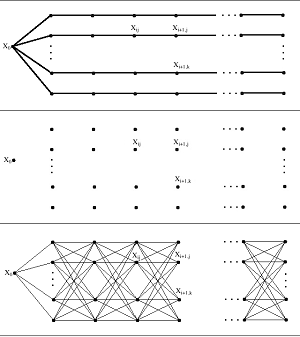
\includegraphics[width=7cm]{mesh_figure.png} 
		\caption{Mesh \label{fig:mesh}}
	\end{center}
\end{figure}


The weights are related to the probability density function. Intuitively, given a node $(i,j)$, and according to the SDE (1), some $(k,j+1)$ are more likely to be reached by the stock path than others. An important issue of the stochastic mesh method is to determine those weights. 

\subsection{Likelihood Ratio Weights}

Suppose that we want to evaluate the following $C(t_{i+1}, x) = \mathbb{E}[h(t_{i+1},X_{i+1})| X_i = x]$ conditional expectation where $h$ is smooth enough to ensure the existence. 
Let us denote by $(f(t_i, X_i, X_{i+1}))_{i \in {1, ..., m-1}}$ the transition densities of Markov Chain $(X_i)_{i \in {1, ..., m}}$, and $g\left(t_i, X_i\right)$ density function of $X_i$. 
Then, by definition, 
\begin{equation}
\mathbb{P}[X_{i+1} \in A|X_i=x] = \int_{A}^{}f_i(x, y)dy  \notag
\end{equation}
which leads to


\begin{eqnarray}
\mathbb{E}[h(t_{i+1},X_{i+1})|X_i = x] &=& \int h(t_{i+1},y) f(t_i, x, y)dy \notag \\
&=& \int h(t_{i+1},y)  \frac{f(t_i, x, y)}{g(t_{i+1}, y)}g(t_{i+1}, y)dy \notag \\
&=& \mathbb{E}[h(t_{i+1},X_{i+1})  \frac{f(t_i, x, X_{i+1})}{g(t_{i+1}, X_{i+1})}]
\end{eqnarray}

Defining now 

\begin{eqnarray}
\hat{C}(t_i, X_{i,j}) &=& \frac{1}{N} \sum_{k=1}^{N} h(t_{i+1},X_{i+1}) \omega_{i,j}^k \notag \\
\omega_{i,j}^k & = &\frac{f(t_i, X_{i, j}, X_{i+1, k})}{g(t_{i+1}, X_{i+1, j})} \notag
\end{eqnarray} 

$\widehat{C}$ is an unbiased estimator of $C$ when $N\rightarrow \infty$, with a convergence rate of $\mathcal{O}(\frac{1}{\sqrt{N}})$. 

Using definition of $g$, 

\begin{eqnarray}
g(t_{i+1}, X_{i+1}=y) &=& \int f(t_i, x, y) g(t_i, x)dx \notag \\
&=& \mathbb{E}[f(t_i, X_i, y)]
\end{eqnarray}

Finally, using a second time a Monte-Carlo estimator for the previous density function, we simulate the weights by : 

\begin{equation} \label{eq:mesh}
\omega_{i,j}^k =  \frac{f(t_i, X_{i, j}, X_{i+1, k})}{\frac{1}{N} \sum_{j=1}^{N}f(t_i, X_{i, j}, X_{i+1,k})} \notag
\end{equation}


As a reminder, our main problem is calculation of : 


\begin{empheq}[left = \empheqlbrace]{align}
&\mathbb{E}[Y_{i+1}|X_i] \notag\\
&\mathbb{E}[Y_{i+1}\Delta B_{i+1}|X_i] \notag
\end{empheq}

So adapting our previous calculus

\begin{empheq}[left = \empheqlbrace]{align}
\widehat{Y_{i, j}} &= \frac{1}{N} \sum_{k=1}^{N} \widehat{Y}_{i+1, k} \omega_{i,j}^k \notag \\
\widehat{Z}_{i, j} &= \frac{1}{N} \sum_{k=1}^{N} \widehat{Y}_{i+1, k}\Delta B_{i+1, j}^k \omega_{i,j}^k \notag
\end{empheq}

are highly biased estimators of our two conditional expectations (see \cite{glasserman:broadie} for proof)


\begin{Rem}
	The reader can refer to \cite{glasserman:amoption} for another method for weights computation, based on optimization of entropy function. 
\end{Rem}

\subsection{Limits}


Mesh Method presents two main drawbacks, especially when used in higher dimension. 
First, computing the weights requires transition densities, which is not always available (can be computed approximatively though, using the Euler scheme, when SDE is not a geometric Brownian motion). 
Second, its time complexity of $\bigO(dmN^2)$, where $d$ is the dimension, $m$ the number of steps used for discretization, and $N$ the number of samples, limits the use of big samples especially. 
For instance, $10^4$ particles would require in Python 10GB of memory in dimension four. Indeed, one float takes 24 bytes in memory, so generating $10^4$ particles requires at every step the construction of an $N\times N$ matrix of weights, taking then $24\times N^2 = 2.4.10^9$ bytes in memory. Hence, working with a 4-dimensional problem would require 10GB memory, way more than an average capacity of 4GB. 

\section{Least Square Monte-Carlo}

A Least Square Monte-Carlo can be used for the simulation of conditional expectation of the form $\mathbb{E}[Y|X]$, when $X$ and $Y$ are square integrable random variables, and a set of numerical values $(X,Y)$ is available. 

Longstaff and Schwartz made this method popular in financial mathematics for the pricing of American Options, which is build upon a basis projection, i.e upon the statement $\mathbb{E}[Y|X] = h(X)$. 

$h$ minimizes what we call a least square function, i.e. 

\begin{equation}
h = \arg \min\{\mathbb{E}[|Y - f(X)|^2] \quad,  f \enskip \text{such that} \quad \mathbb{E}[|f(X)|^2]<\infty\}
\end{equation}

This infinite-dimensional problem can be restricted to smaller set of functions to look for. 
Our simulations for one asset will be using polynomials. 

Although very easy to implement in practice, this kind of function basis has a
major flaw. For a given number of particles it is not easy to find an optimal degree
of the functional basis. This is due to rare events that
the polynomials try to fit, leading to some oscillating representation of the function (see below \ref{fig:lsm_regression}). 


\begin{figure}[H]
	\centering
	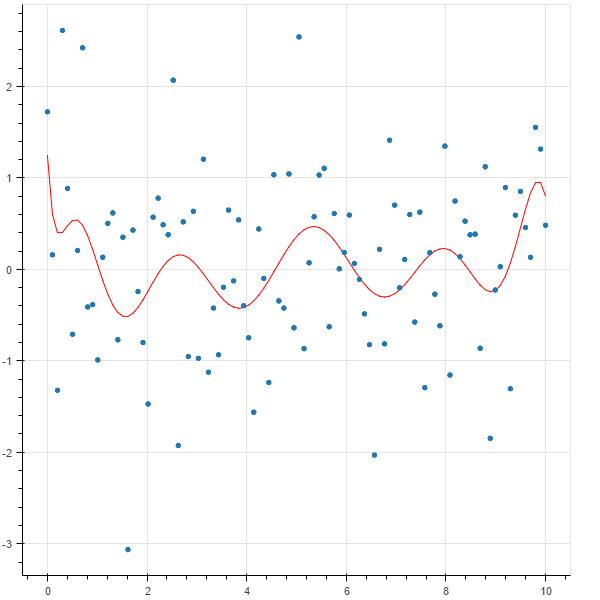
\includegraphics[scale = 0.5]{polynomial.png}
	\caption{Example of polynomial fitting with degree 10 on a random dataset \label{fig:lsm_regression}}
	
\end{figure}

\begin{Rem}
	We will only use this method for one dimensional example. Indeed, basis projection using polynomials in higher dimension would require too much computational time, and one can show time complexity with number of features $d$ is $\bigO (d^2)$ ...
\end{Rem}

\section{Random Forest Regression}

	
\begin{minipage}{\textwidth-2\fboxrule-2\fboxsep\relax}
	The following section is the main contribution to BSDE analysis, as it uses a machine learning method, Random Forest (Randomized Tree Decision), for the regression step. 
	We will first focus on a quick analysis of decision trees. From there, we will explain Randomized Trees methods using a housing market data in Iowa. We will mainly focus on  hyperparameters tuning and complexity of the different Random Trees methods. 
\end{minipage}


\subsection{Decision Tree}
Machine learning research has given plenty of new methods for classification and regression problems. Most effective remain the tree based methods, intuitive and reliable for almost any kind of data. 

Following Gilles Louppe (\cite{glouppe:rf}) 

\begin{defn}
	A tree is a graph $G = (V, E)$ in which any two vertices (or
	nodes) are connected by exactly one path.
\end{defn}

\begin{defn}
	A rooted tree is a tree in which one of the nodes has been
	designated as the root. In our case, we additionally assume that a rooted tree
	is a directed graph, where all edges are directed away from the root.
\end{defn}

\begin{defn}
	If there exists an edge from t1 to t2 (i.e., if (t1, t2) 2 E)
	then node t1 is said to be the parent of node t2 while node t2 is said to be a
	child of node t1.
\end{defn}

\begin{defn}
	In a rooted tree, a node is said to be internal if it has one
	or more children and terminal if it has no children. Terminal nodes are also
	known as leaves.
\end{defn}

\begin{defn}
	A binary tree is a rooted tree where all internal nodes have
	exactly two children.
\end{defn}


\begin{figure}[t!]
	\centering
	\begin{subfigure}[t]{0.3\textwidth}
		\includegraphics[width=\textwidth]{decision_tree.png}
		\caption{}
		\label{fig:gull1} %  
	\end{subfigure}
	~~~~~~~~~~~~~~~
	\begin{subfigure}[t]{0.3\textwidth}
		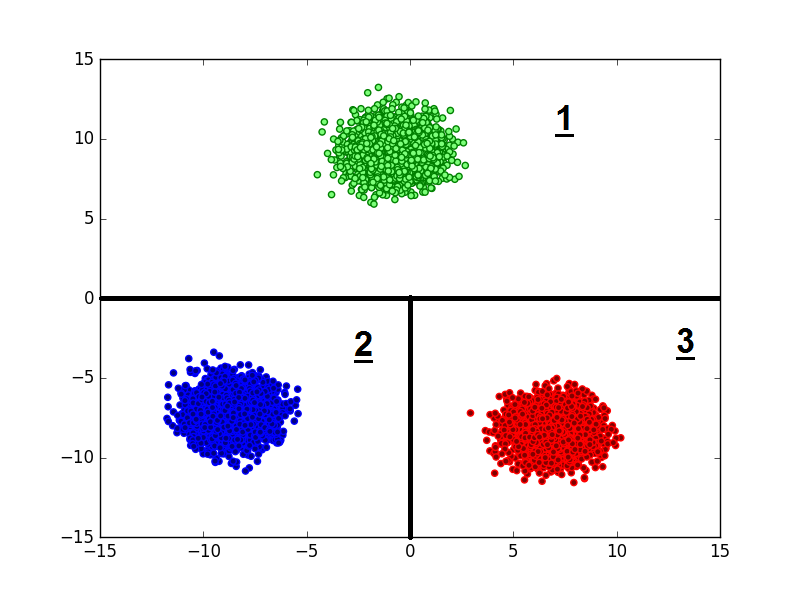
\includegraphics[width=\textwidth]{classification_presentation.png}
		\caption{}
		\label{fig:gull}
	\end{subfigure}
	\caption{A binary tree built for a classification $(1, 2, 3)$ problem from an input space $[-15, 15] \times [-15, 25]$}
\end{figure}


\subsection{Randomized Forest}

\begin{Def}
	Random Forests is a tree based regression and classification method. 
	Given a dataset $\left(x_i, y_i\right)_{1 \leq i \leq N}$, this method is based on generating multiple binary decision trees of the given dataset, and taking the average (regression) or Gini criterion (classification) as expected output for a new input $\tilde{x}_i$.
	
\end{Def}

\begin{Rem}
The algorithm could be written as 
	
\begin{algorithm}[H]
	\caption{General idea of the algorithm}\label{algo:RFgeneral}
	\begin{algorithmic}[1]
		\Procedure{RandomForest}{}
		\For {a bootstrap sample from the data}
		\State fit a regression/classification tree
		\EndFor
		\State Combine by voting(classification) or averaging(regression)
		\EndProcedure
	\end{algorithmic}
\end{algorithm}

\end{Rem}


\subsubsection{Growing one tree}

\begin{algorithm}[H]
	\caption{Growing a tree in the Random Forest}\label{algo:RFsplit}
	\begin{algorithmic}[1]
		\Procedure{GrowTree}{}
		\For{a node}
		\State select K variables out of all d available 
		\State Find the best split 
		\State Generate children
		\EndFor
		\EndProcedure
	\end{algorithmic}
\end{algorithm}


\subsubsection{Splitting nodes}

Growing one tree requires splitting nodes. Different criteria are used given regression or classification. 

\begin{itemize}
	\item  Regression

Residual Sum of Square (RSS) is among criteria used for splitting nodes in regression. 
This can be written as : 

\begin{displaymath}
RSS = \sum_{i \in \text{left node}}^{} (y_i - y_L)^2 + \sum_{R \in \text{right node}}^{} (y_i - y_R)^2
\end{displaymath}

where $y_L$ and $y_R$ are the  mean y-value for left node and right node respectively.

%
%
%\begin{figure}[h!]
%	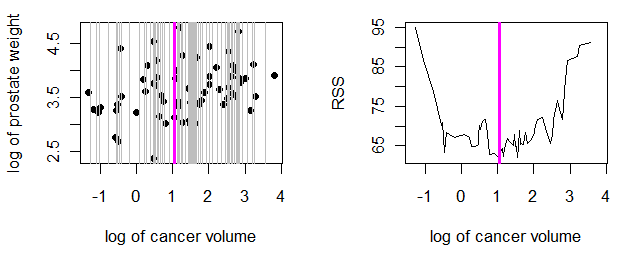
\includegraphics[scale=0.8]{time_complexity/sorting_split.png}
%	\caption{Choosing the best vertical split using RSS measure \label{figure:RFsplit}} 
%\end{figure}

	\item Classification
	
	
	We call Gini criterion 
	
	\begin{displaymath}
	Gini = n_L\sum_{k \in {1, \cdots, K}}^{} p_{k_L} ()1- p_{k_L}  + n_R\sum_{k \in {1, \cdots, K}}^{} p_{k_R} ()1- p_{k_R}
	\end{displaymath}
	
	Where $p_{k_L}$ and $p_{k_R}$ are the proportion of class k in left node and right node respectively.
\end{itemize}


Hence, using these criterion to grow multiples trees gives us the Randomized Forest.


\section{Derivative}

Another method we will use in the simulations is the derivative one. 
As explained in 1-BSDE section, $(Y_t = u(t;X_t);Z_t =\sigma(t,x)^T D_xu(t;X_t))$ is solution to (8), with $u$ solution to semi-linear PDE (9).  
Given our algorithm process

%\begin{comment}

\begin{algorithm}[H]
\caption{BSDE Algorithm}\label{algo:derivative1}
\begin{algorithmic}[1]
		\Procedure{BSDE}{}
		\For{$t \in \{T-1, \cdots, 0\}$}
		\State $Z[t] =\frac{1}{\Delta t}\mathbb{E}_t[Y_{t + 1} \Delta B_t]$
		\State $Y[t] = \mathbb{E}_t[Y_{t+1} +  f(t,X_t, Y_{t+1}, Z_t)\Delta t]$
		\EndFor
		\EndProcedure
\end{algorithmic}
\end{algorithm}

for all $t$ we can compute once the previous algorithm, and enhance it by taking $Y_t = \phi(t, X_t)$ with $\phi$ smooth enough to be derivable, and derive from there $Z_t = \nabla \phi (t, X_t)$. We repeat the process $M$ times, as one would derive for a Picard iteration.


\begin{algorithm}[H]
	\caption{BSDE Algorithm}
	\label{algo:derivative2}
	\begin{algorithmic}[1]
		\Procedure{BSDE}{}
		\For{$t \in \{T-1,\cdots, 0\}$}
		\State $Z[t] =\frac{1}{\Delta t}\mathbb{E}_t[Y_{t + 1} \Delta B_t]$ \text{by RandomForest for instance}
		\State $Y[t] = \mathbb{E}_t[Y_{t+1} +  f(t,X_t, Y_{t+1}, Z_t)\Delta t]$
		\For {i = 1:M}
		\State  \text{Get $\phi$ such that} $Y_t \sim \phi(t, X_t)$
		\State  $Y_{new} = \phi(t, X_t)$
		\State 	$Z_{new} = \nabla \phi(t, X_t)$ \text{gives a new smoother $Z$}
		\State  $Y[t] = \mathbb{E}_t[Y_{t+1} +  f(t,X_t, Y_{t+1}, Z_{new})\Delta t]$
		\EndFor
		\EndFor
		\EndProcedure
	\end{algorithmic}
\end{algorithm}

%\end{comment}
\noindent
$Z$ being a very noisy process, due to the factor $\frac{\Delta B_t}{\Delta t}$, especially when $\Delta t \rightarrow 0$, it seemed relevant to get the smoothest approximation possible. 
\noindent
In our simulation, we use a kernel regression to recover a smooth $\phi$ function. 
Kernel regression consists on a sum of smooth functions, each one giving an approximation around a point $(X_i, Y_i)$.
\noindent
We assume that points  that  are  close  together  are  similar,  a  kernel defines  then weights  that  decrease  in  a  smooth  fashion  as  one  moves  away from the target point.
 
\noindent
Denoting $K\left(\frac{X - X_i}{l}\right)$ the kernel function for the point $(X_i, Y_i)$, where l controls the scale and length,  we define the weight $\omega(X, X_i) = \frac{K(\frac{X - X_i}{l})}{\sum_{i=1}^{N} K(\frac{X - X_i}{l})}$ such that $\phi(X) = \sum_{i=1}^{N} \omega(X, X_i)Y_i$. 

\begin{Rem}
	$\sum_{i=1}^{N} \omega(X, X_i) = 1$
\end{Rem}

\noindent
We use in our simulations a Gaussian Kernel with scaling parameter $l$, i.e 

\begin{displaymath}
K\left(\frac{X - X_i}{l}\right) = \exp^{- \frac{||X - X_i||^2}{2l^2}}
\end{displaymath} 


\begin{Ex}	
	Let $Y$ be a random variable defined by $Y_x = \sin(\frac{x}{10}) + \frac{x}{50} + 0.3 \exp^{-x} + \epsilon$, where $\epsilon \sim \mathcal{N}(0, 0.09)$ and $x \in \left[0, 100\right]$.
	Let $X$ be a linear space division of $\left[0, 100\right]$ interval with 200 points.
	Applying a Kernel Regression on $\left(X, Y_X\right)$ gives
	
	\begin{figure}[H]
		\begin{center}
			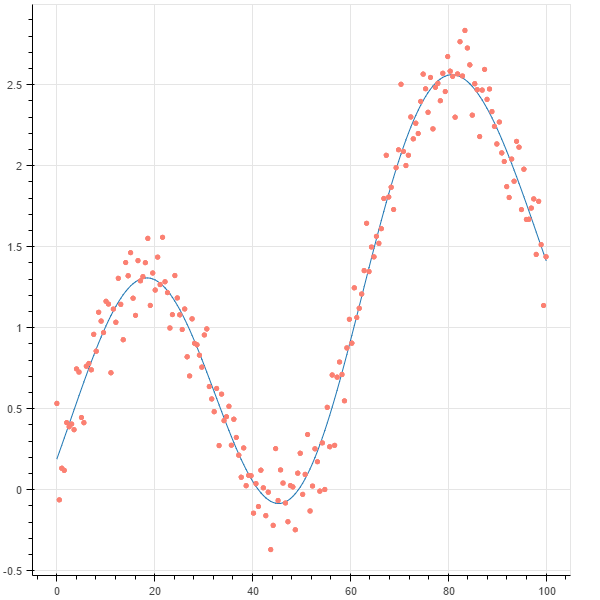
\includegraphics[scale=0.5]{kernel_regression/example.png} 
			\caption{Example of Gaussian Kernel Regression}
		\end{center}
	\end{figure}
	\newpage
\end{Ex}

\begin{Rem}
	In one dimension, this algorithm requires the construction of an $N \times N$ matrix of weights. To avoid this $\bigO(N^2)$ we can consider the '$\mathcal{K}$ Nearest Neighbours' (KNN) instead of all the points when computing the weights. 
	Hence, $\phi(X) = \sum_{i \in \mathcal{S}_{\mathcal{K}}} \omega(X, X_i)Y_i $, where $\mathcal{S}_{\mathcal{K}}$ is a subset of $\left\lbrace 1, \cdots, N \right\rbrace$ with indices of the KNN.
\end{Rem}


\section{Picard Iteration}

The noisy $Z_t$ process can be better approximated iteratively using a Picard iteration. This idea has been inspired from E.Gobet \cite{gobet:picard} and was added as an option in our code. 
Hence, the backward algorithm process with Picard iteration 
	
	
\begin{algorithm}
	\caption{BSDE Algorithm with Picard iteration}
	\label{algo:picard}
	\begin{algorithmic}[1]
		\Procedure{BSDE}{}
		\For{$t \in \{T-1,\cdots, 0\}$}
		\State Y\_new = 0
		\State $Z_t =\frac{1}{\Delta t}\mathbb{E}_t[Y_{t + 1} \Delta B_t]$ \text{by RandomForest for instance}
		\State $Y_t = \mathbb{E}_t[Y_{t+1} +  f(t,X_t, Y_{t+1}, Z_t)\Delta t]$
		\For {\_\_ = 1:n\_picard}
		\State  $Z_t =\frac{1}{\Delta t}\mathbb{E}_t[(Y_{t + 1} - Y_t)\Delta B_t]$
		\State  $Y_{new} = \mathbb{E}_t[Y_{t+1} +  f(t,X_t, Y_{t+1}, Z_t)\Delta t]$
		\State  $Y_t = Y_{new}$
		\EndFor
		\EndFor
		\EndProcedure
	\end{algorithmic}
\end{algorithm}
	
\section{Time Complexity}		
	
	Time complexities presented below in table \ref{table:t_complexity} differ with the method used. 
	Hence, the preferred LSM when dimensions are low, as every step is asymptotically $\bigO(N)$.
	Then comes mesh and derivative methods, using $N\times N$ matrices, which barres us from using high amount of samples. 
	Finally, as explained in Appendix B, Random Forest time complexity can not be obtained theoretically, but lower bounds and upper bounds exist, depending on number of trees generated and number of features used. 
	
	\begin{table}[H]
		\centering
	
		\begin{tabular}{l|c}
			\hline
			 Mesh & $\bigO(dn_{picard}mN^2)$  \\ \hline
			Random Forest $\footnote{\text{cf Appendix A for more precision}}$ \\ (worst case - best case) & $\bigO(n_{trees}Kn_{picard}mN^2\log(N))$\\ &  $\bigO(n_{trees}Kn_{picard}mN\log(N)^2) $ \\ \hline
			Derivative &  $\bigO(Kn_{picard}mN^2)$ \\ \hline
			 LSM &  $\bigO (d^2n_{picard}mN)$ \\ \hline
			
		\end{tabular}
		\caption{Time Complexity with number of samples M, number of paths m, number of picard iteration $n_{picard}$, dimension d, K the number of selected features\label{table:t_complexity}, and $n_{trees}$ the number of trees in the Random Forest}
	
	\end{table}
 

\chapter{Applications}

\section{Introduction}

The following simulations are computed on Python 3.5, with ten CPUs available in the Department of Applied Probability and Statistics in NUS. 

Each example relies on a theoretical solution, or a comparison found in BSDE literature. 

We will give for every example the solution given by the previous cited methods, with its $95\%$ confidence interval, and the average time. 
When not specified, we run \#30 simulations for every average given, and use a Picard iteration number of three. 

We apply BSDE theory on European and American option pricing, respectively on one and multiple assets.

Assets follow a Black-Scholes model 

\begin{displaymath}
\frac{dX_t^i}{X_t^i} = (\mu^i_t - q^i) dt + \sigma^i_t dB_t^i
\end{displaymath}

where $\mu$ denotes the drift rate, $\sigma$ the volatility, $q$ the dividend (will be equal to zero in application, unless stated by the author), i the i'th assets ($i \in \left\lbrace1, d\right\rbrace$)and $X$ the asset price.

First example analysis will be exhaustive, especially comparison of  different methods implemented for regression step.
For instance, we will detail how Random Forest parameters have been calibrated for a European call option with different interest rates, and will follow the same idea for the next applications.    

Moreover, all the  results in table are given with a standard deviation. 

\subsection{Bid-ask model}

Suppose the dynamic of the underlying assets to be : 

\begin{align}
\frac{dX_t^i}{X_t^i} & = (\mu^i_t - q^i) dt + \sigma^i_t dB_t^i\\
\left\langle dB_t^i,dB_t^j \right\rangle &= \left\{ \begin{array}{ll}
										dt \quad \text{if} \quad i=j \\
								\rho dt \quad \text{else} 
								\end{array}
								\right.
\end{align}

and let the agent be able to lend ($r$) and borrow ($R$) money using two market accounts. 

\begin{equation}
\left\{
\begin{aligned}
d\alpha_t &= R \alpha_t dt\\
d\beta_t &= r \beta_t dt\\
\end{aligned}
\right.
\end{equation}

\noindent
Let $Y_t$ be the portfolio value at time $t$ and $\Phi^i_t$ the amount of shares invested in stock $X_t^i$ at time $t$. Intuitively, if the difference $Y_t - \sum_{i = 1}^{d} \Phi^i_t$ is positive, the agent can lend to the bank. Inversely, if this difference is negative, the agent would rather borrow money. 
\noindent
Hence the variations of $dY_t$

\begin{displaymath}
dY_t = \sum_{i = 1}^{d} \Phi^i_t \frac{dX^i_t}{X^i_t} + (Y_t - \sum_{i = 1}^{d} \Phi^i_t)^+rdt - (Y_t - \sum_{i = 1}^{d} \Phi^i_t)^-Rdt
\end{displaymath}


We get then the following BSDE

\begin{equation}
-dY_t = f(t,Y_t,Z_t)dt - Z_tdW_t  
\end{equation}

where 

\begin{equation}
\left\{
\begin{aligned}
&f(t,Y_t,Z_t)  =   Z_t\theta - rY + (R-r)(Y- \sum_{i=1}^{d}(\sigma^{-1}Z_t)_i)^-\\
&Z_t  = \sigma\Phi_t\\
&\theta = \sigma^{-1}(\mu - r)\mathbbm{1}
\end{aligned}
\right.
\end{equation}

Here, $\mathbbm{1}$ is the unit vector of dimension $d$ and $\Phi_t$ the vector of investments $\left(\Phi^i_t\right)_i$.

\subsection{Credit Valuation Adjustment (CVA)}

Using same notations than Guyon and Labordère \cite{GuyonLabordere:cva}, CVA can be transformed into a BSDE problem

\begin{displaymath}
\left\{
\begin{aligned}
&-dY_t = f(t,Y_t,Z_t)dt - Z_tdW_t \\
&f(t,Y_t,Z_t)  =  \beta (Y_t^+ - Y_t)
\end{aligned}
\right.
\end{displaymath}

where $\beta = \lambda_C(1 - R)$ with $R$ the recovery rate (usually equal to 0.4), and $\lambda_C$ the intensity of the Poisson jump process associated to the CVA problem(see \cite{GuyonLabordere:cva}) ,
with the corresponding semi-linear PDE 

\begin{eqnarray}
\partial_t u + \mathcal{L}u + \beta(u^+ -u) &=& 0 \notag \\
u(T, x) &=& g(x) \notag
\end{eqnarray}

where $\mathcal{L}$ is the Itô generator of a diffusion $X_t$.

There is no process $Z$ to regress here, but we will analyse how Random Forest performs on $\E_t[Y_{t+ \Delta t}^+]$, comparing the results to Guyon and Labordère(\cite{GuyonLabordere:cva}). 



\section{One dimension}

\subsection{Bid-ask European call option} 

Referring to Gobet, Lemor and Warin's simulations in \cite{gobet:example}, we take the following numerical values 

\begin{table}[H]
	\centering
	\begin{tabular}{ |l|c|c|c|c|c|c|}\hline
		$X_0$ & $K$ & $\sigma$ & $r$ & $R$ & $\mu$ \\ \hline
		100   & 100  & 0.2 & 0.04 & 0.06 & 0.06      \\ \hline
		
	\end{tabular}
\end{table}

We compute the pricing of an European call (i.e pay-off $(X_T - K)^+$) on a single asset associated. This problem has a theoretical solution, given by the Black-Scholes model with $R$ used as free-risk rate. 
Indeed, to hedge himself, the financial seller will borrow money to buy assets, hence the use of $R$. 

\begin{figure}[H]
	\centering
	
	\begin{subfigure}[t]{0.3\textwidth}
		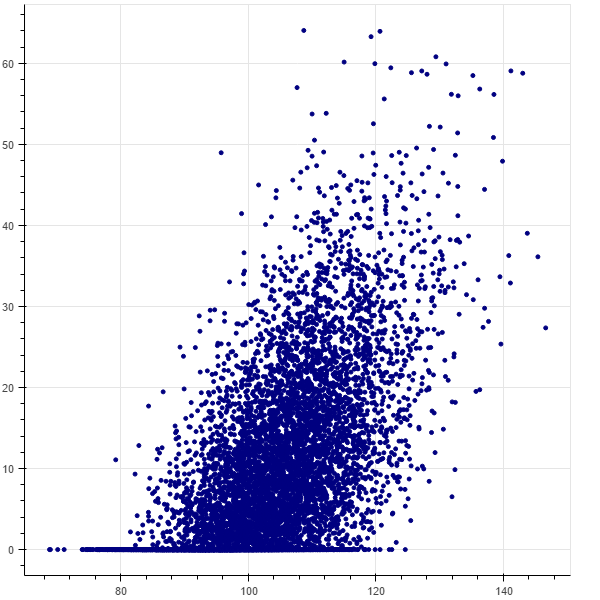
\includegraphics[width=\textwidth]{RF_analysis/Y_X.png}
		\caption{$Y_{t}$ against $X_{t-\Delta t}$}
		\label{fig:Y_X} %  
	\end{subfigure}
	~~~~~~~~~~~~~~~
	\begin{subfigure}[t]{0.3\textwidth}
		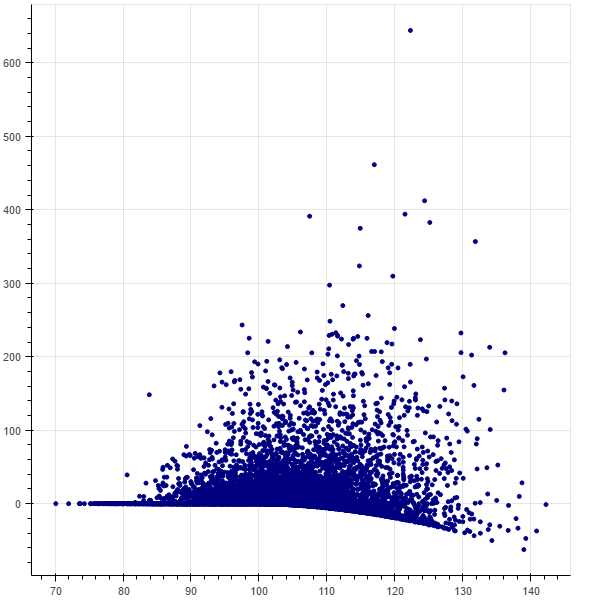
\includegraphics[width=\textwidth]{RF_analysis/Z_X.png}
		\caption{$Y_{t}\frac{\Delta B_t}{\Delta t}$ against $X_{t-\Delta t}$}
		\label{fig:Z_X}
	\end{subfigure}

	\caption{Regression at time $t=T- \Delta t$ \label{fig:plotY_Z}}
\end{figure}


figure \ref*{fig:plotY_Z} shows the first regression step implied by BSDE algorithm. We can notice the noisy process on the right figure due to $\frac{\Delta B_t}{\Delta t}$ term. 
The bigger the difference between the two rates, the more important the approximation error is on $Z_t$ process. 
 
 
 \subsubsection{LSM}

Main parameter when having polynomial basis projection is the degree. The following table gives the simulation results according to number of samples and this degree parameter. 


\begin{table}[H]
	\centering
	\caption{LSM}
	\label{table:lsm}
	\begin{tabular}{|l|c|c|c|c|}
		\hline
		degree & N = 100           & N = 1000          & N = 10000         & N = 100000        \\
		\hline
		1& 7.166 (1.004) & 7.136 (0.24)  & 7.229 (0.084) & 7.242 (0.032) \\ \hline
		2& 7.156 (0.936) & 7.339 (0.326) & 7.254 (0.106) & 7.272 (0.025) \\ \hline
		3& 7.296 (0.834) & 7.191 (0.319) & 7.191 (0.097) & 7.17 (0.029)  \\ \hline
		4& 7.194 (0.889) & 7.24 (0.354)  & 7.17 (0.106)  & 7.177 (0.027) \\ \hline
	5& 	7.222 (0.981) & 7.159 (0.248) & 7.155 (0.074) & 7.168 (0.029) \\ \hline
		6& 7.225 (0.893) & 7.198 (0.298) & 7.164 (0.081) & 7.155 (0.026) \\ \hline
	7& 	7.188 (1.069) & 7.143 (0.319) & 7.145 (0.085) & 7.168 (0.031) \\  \hline
	8& 	7.368 (0.933) & 7.071 (0.258) & 7.154 (0.089) & 7.164 (0.032) \\  \hline 
	9& 	7.45 (1.034)  & 7.156 (0.302) & 7.164 (0.091) & 7.163 (0.034) \\  \hline
	10& 	6.984 (0.986) & 7.227 (0.348) & 7.18 (0.086)  & 7.16 (0.025)  \\  \hline
	11& 	7.188 (1.093) & 7.157 (0.266) & 7.195 (0.104) & 7.169 (0.029) \\  \hline
	12& 	7.187 (0.883) & 7.141 (0.19)  & 7.166 (0.085) & 7.164 (0.026) \\ 
		\hline
		\hline
	\end{tabular}
\end{table}


Paradoxically, accuracy does not increase with polynomial degree. Even if approximation is increased for central data points, peripheral points can undergo high variance issues (cf \ref{figure:poly} below).

Theoretical price of 7.15 is within reach with 100.000 samples and degree 6. 

\begin{figure}[H]
	\centering
	\begin{subfigure}[t]{0.3\textwidth}
		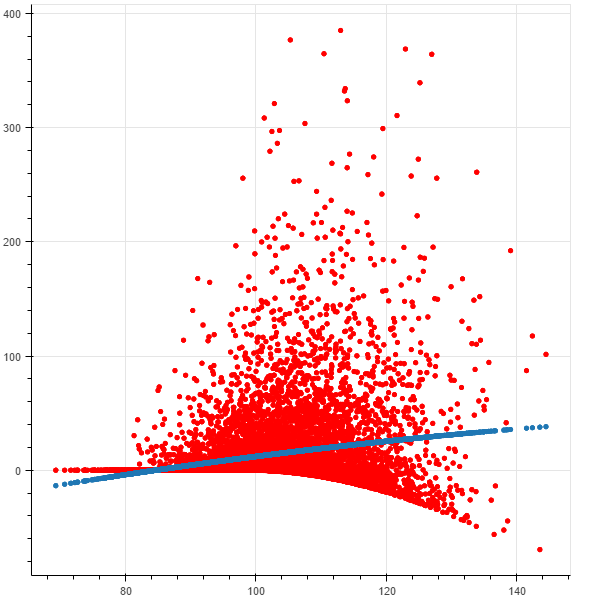
\includegraphics[width=40mm]{lsm/l=2.png}
		\caption{d =2}
		\label{fig:a} %  
	\end{subfigure}
	\begin{subfigure}[t]{0.3\textwidth}
		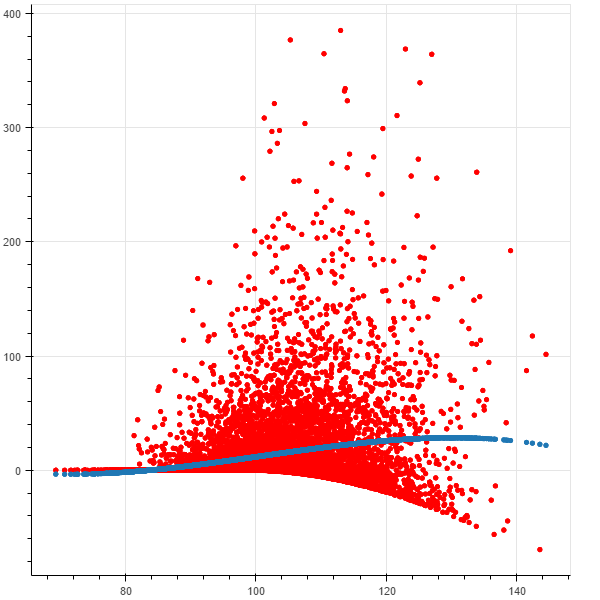
\includegraphics[width=40mm]{lsm/l=3.png}
		\caption{d=3}
		\label{fig:b}
	\end{subfigure}
	\begin{subfigure}[t]{0.3\textwidth}
		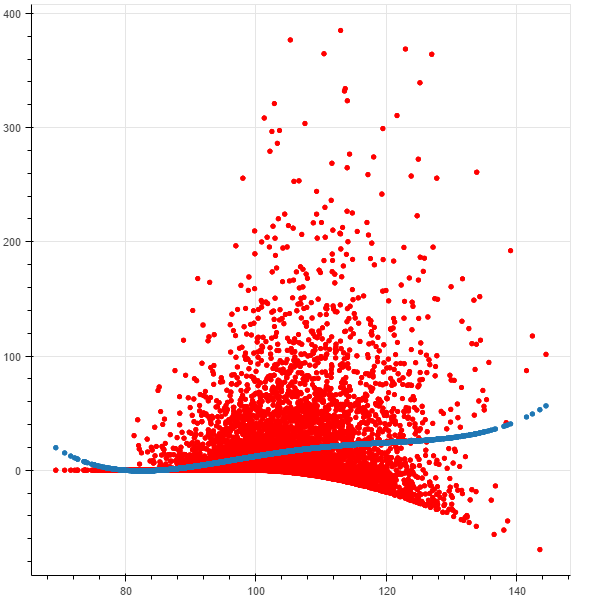
\includegraphics[width=40mm]{lsm/l=4.png}
		\caption{d=4}
		\label{fig:c}
	\end{subfigure}	
	
	\begin{subfigure}[t]{0.3\textwidth}
		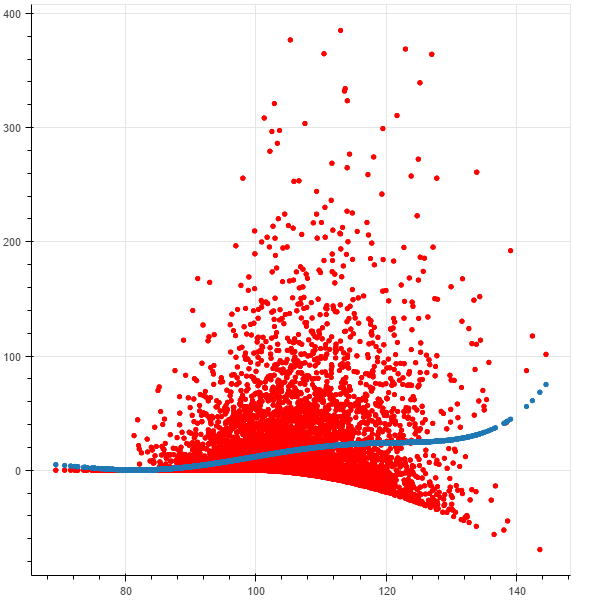
\includegraphics[width=40mm]{lsm/l=5.png}
		\caption{d=5}
		\label{fig:d}
	\end{subfigure}
	\begin{subfigure}[t]{0.3\textwidth}
		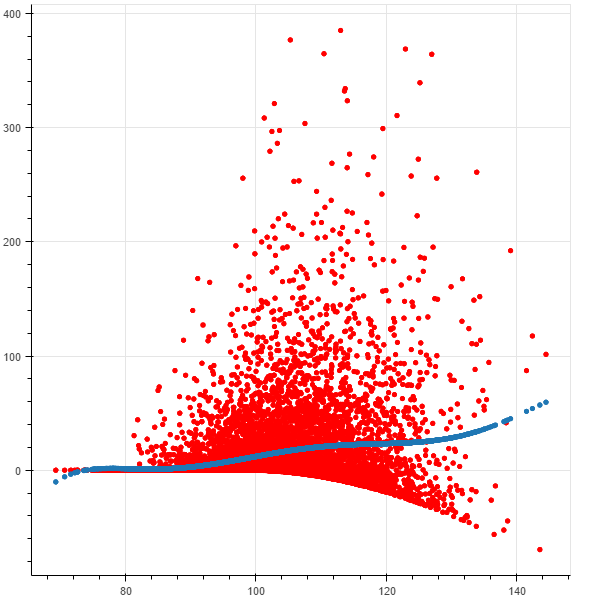
\includegraphics[width=40mm]{lsm/l=6.png}
		\caption{d=6}
		\label{fig:c}
	\end{subfigure}	
	\begin{subfigure}[t]{0.3\textwidth}
		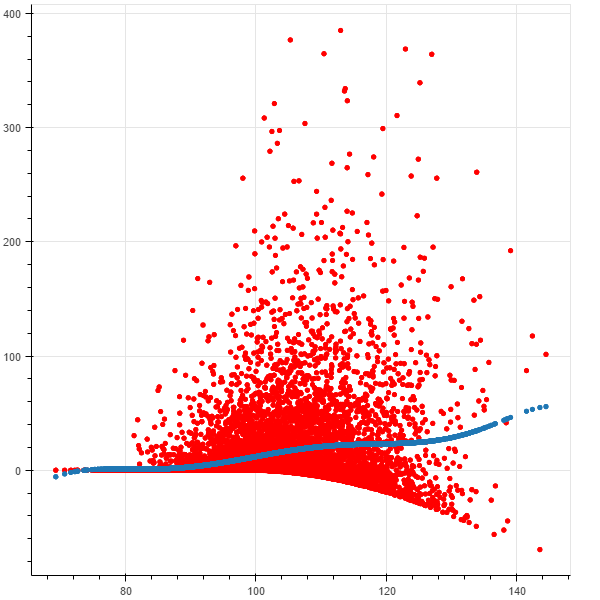
\includegraphics[width=40mm]{lsm/l=7.png}
		\caption{d=7}
		\label{fig:d}
	\end{subfigure}

	\begin{subfigure}[t]{0.3\textwidth}
		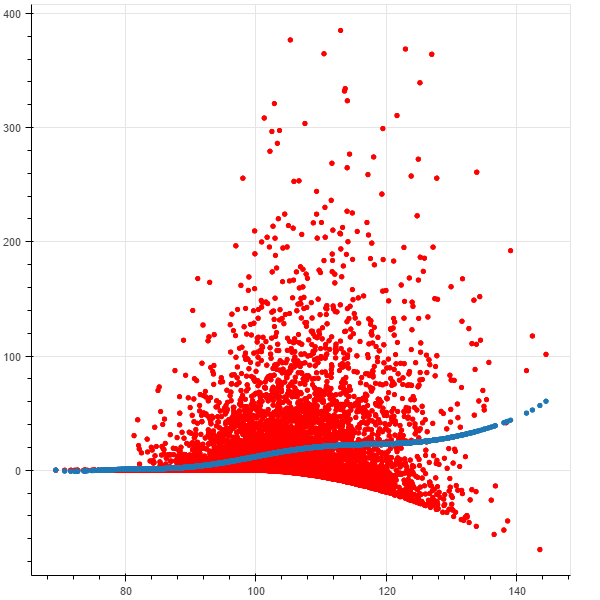
\includegraphics[width=40mm]{lsm/l=8.png}
		\caption{d=8}
		\label{fig:d}
	\end{subfigure}
	\begin{subfigure}[t]{0.3\textwidth}
		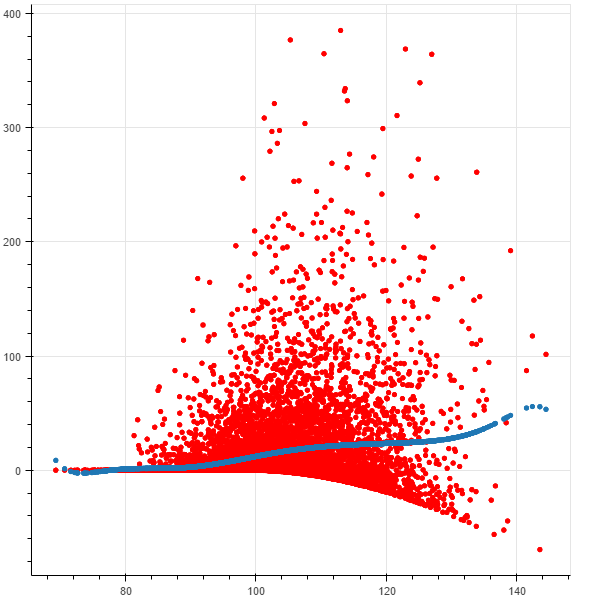
\includegraphics[width=40mm]{lsm/l=9.png}
		\caption{d=9}
		\label{fig:c}
	\end{subfigure}	
	\begin{subfigure}[t]{0.3\textwidth}
		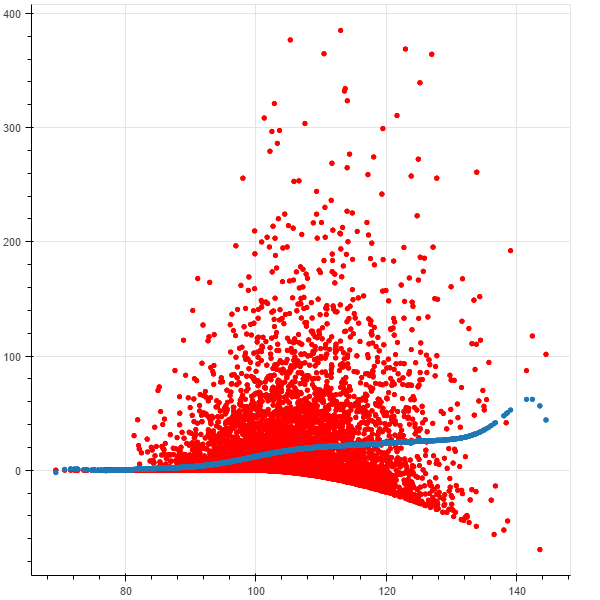
\includegraphics[width=40mm]{lsm/l=10.png}
		\caption{d=10}
		\label{fig:d}
	\end{subfigure}

	\caption{Display of the regression step using LSM method (in blue) with different polynomial degrees and display of $Y_{t}\frac{\Delta B_t}{\Delta t}$ with respect to, both with respect to $X_t$ \label{figure:poly}}
\end{figure}

Regression of noisy process $Z$ with polynomials does not cover all the noisy process. Moreover, peripheral points are confronted to high variance depending on the degree.


 \subsubsection{Mesh}

With Black-Scholes formulation, density function takes the following expression 

\begin{align}
f(t_i, X_{i, j}, X_{i+1, k}) & = \frac{1}{\sigma \sqrt{\Delta t}} \phi\left(\frac{\ln(\frac{X_{i+1, k}}{X_{i, j}} - (\mu - \frac{1}{2} \sigma ^2))}{\sigma \sqrt{\Delta t}} \right)
\end{align}


We inject then in weights expression(\ref{eq:mesh}) and draw results in following table \ref{table:mesh}. Prices computed are given with respect to N samples and m discretization time.

\begin{table}[H]
	\centering
	\caption{Mesh with number of paths and time discretization}
	\label{table:mesh}
	\begin{tabular}{|l|c|c|c|c|c|}
		\hline
		m & N = 100           & N = 1000    &N = 2000&   N = 4000         & N = 10000 \\ 
		\hline
		4 & 7.249 (0.951) & 7.174 (0.309) & 7.145 (0.219) & 7.151 (0.153) & 7.152 (0.096) \\ \hline
		6 &  7.184 (1.051) & 7.166 (0.324) & 7.155 (0.214) & 7.157 (0.154) & 7.152 (0.098) \\ \hline
		8 & 7.17 (0.97)   & 7.143 (0.328) & 7.163 (0.235) & 7.16 (0.156)  & 7.157 (0.098) \\ \hline
		10  &7.186 (1.109) & 7.19 (0.315)  & 7.141 (0.219) & 7.165 (0.161) & 7.145 (0.099) \\ \hline
		12 & 7.171 (1.015) & 7.147 (0.316) & 7.147 (0.22)  & 7.144 (0.169) & 7.161 (0.101) \\ \hline
		\hline
	\end{tabular}
\end{table}

\begin{Rem}
	As the number of samples increases, standard deviation decreases as expected, and price seems to converge to theoretical 7.15. 
	Moreover, when number of paths is big, like 12, we notice an inaccuracy, due to terms in $\frac{1}{\Delta t}$ becoming bigger, thus making $Z$ even more noisy. 
\end{Rem}

 
 The following figure show one regression using this mesh approximation.
 
\begin{figure}[H]
	\centering
	\captionsetup{width=0.8\textwidth}
	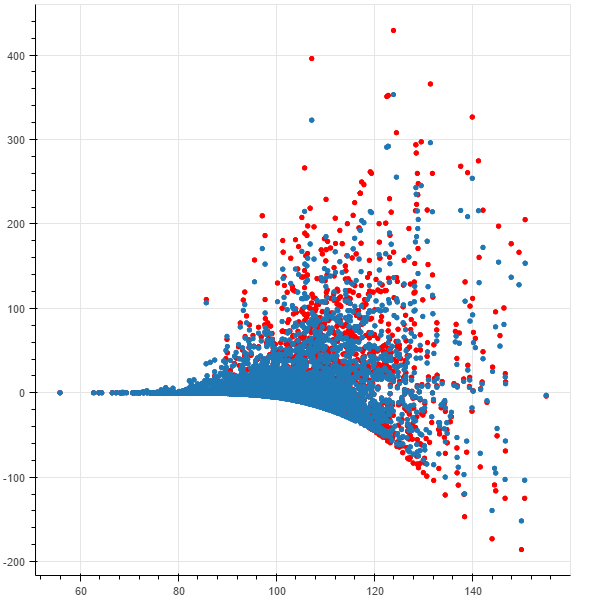
\includegraphics[scale = 0.3]{mesh/mesh.png}
	\caption{Display of the regression step using mesh method (in blue) and display of $Y_{t}\frac{\Delta B_t}{\Delta t}$ (red) , both with respect to $X_t$}
	
\end{figure}


 \subsubsection{Random Forest}




\begin{table}[H]
	\centering
	\caption{Random Forest with number of paths and number of trees generated}
	\label{table:rf1}
	\begin{tabular}{|l|c|c|c|c|c|}\hline
		n\_trees & N = 100           & N = 1000          & N = 10000         & N = 100000 \\ 
		\hline
		10 & 6.917 (0.988) & 6.984 (0.322) & 7.207 (0.117) & 7.238 (0.031) \\ \hline
		50 & 7.187 (1.208) & 7.09 (0.295)  & 7.221 (0.132) & 7.218 (0.026) \\ \hline
		100 & 7.229 (1.057) & 7.069 (0.375) & 7.159 (0.107) & 7.211 (0.036) \\ \hline
		150  & 7.26 (0.921)  & 7.055 (0.307) & 7.202 (0.086) & 7.221 (0.028) \\ \hline
		200 & 6.61 (0.836)  & 7.209 (0.242) & 7.198 (0.103) & 7.226 (0.026) \\ 
		\hline
		\hline
	\end{tabular}
\end{table}

Obviously, the more the number of trees generated, the smaller the variance. Unfortunately, playing only with the number of trees gives a highly biased result. Indeed, with 200 trees and $10^5$ samples, we get $Y_0 = 7.226$, far from the expected $7.15$. 

Referring the reader to Appendix B, multiple sensitive parameters can be the source of this bias. 
We focus on the most sensitive one, the number of maximum leafs allowed in the tree (related then to depth of the tree). 

\begin{Rem}
	Even though generating 200 trees does not provide a better result, Appendix B shows this parameter has to be taken bigger than 150 at least. We will fix it to 200 and try to calibrate the number of maximum allowed leafs. 
\end{Rem}


\begin{table}[H]
	\centering
	\caption{Random Forest with number of samples N and maximum number of leafs(in percentage of N)}
	\label{table:rf2}
	\begin{tabular}{|l|c|c|c|c|}\hline
		max\_leafs & N = 100           & N=1000          & N=10000         & N=50000         \\
		\hline
		5\% & 7.115 (0.795) & 7.027 (0.265) & 7.096 (0.101) & 7.101 (0.036) \\ \hline
		10\% &6.717 (1.031) & 7.023 (0.316) & 7.073 (0.1)   & 7.062 (0.049) \\ \hline
		15\% & 6.767 (0.944) & 7.017 (0.291) & 7.063 (0.117) & 7.069 (0.036) \\ \hline
		20\% &6.796 (0.773) & 7.114 (0.244) & 7.074 (0.078) & 7.101 (0.047) \\ \hline
		25\% &6.922 (0.977) & 7.2 (0.323)   & 7.115 (0.09)  & 7.127 (0.046) \\ \hline
		30\% &6.71 (1.235)  & 7.139 (0.375) & 7.119 (0.092) & 7.159 (0.045) \\ \hline
		35\% &6.881 (1.046) & 7.168 (0.338) & 7.173 (0.109) & 7.192 (0.044) \\ \hline
	40\% &	7.244 (1.146) & 7.182 (0.289) & 7.218 (0.118) & 7.195 (0.041) \\\hline
		45\% &6.981 (0.85)  & 7.243 (0.312) & 7.218 (0.108) & 7.218 (0.04)  \\ \hline
	50\% &	7.281 (1.091) & 7.234 (0.367) & 7.221 (0.091) & 7.222 (0.051) \\ \hline
	55\% &	6.893 (0.954) & 7.246 (0.325) & 7.224 (0.089) & 7.226 (0.05)  \\ \hline
	60\% &	7.164 (0.932) & 7.083 (0.285) & 7.23 (0.109)  & 7.23 (0.051)  \\ \hline
	65\% &	7.069 (0.99)  & 7.239 (0.333) & 7.226 (0.081) & 7.222 (0.042) \\ \hline
	70\% &	7.158 (1.035) & 7.206 (0.378) & 7.247 (0.078) & 7.233 (0.037) \\ \hline
	75\% &	7.211 (1.138) & 7.211 (0.267) & 7.206 (0.107) & 7.215 (0.041) \\ \hline
	80\% &	6.934 (1.027) & 7.291 (0.226) & 7.237 (0.097) & 7.224 (0.05)  \\ \hline
	85\% &	6.878 (1.016) & 7.287 (0.326) & 7.242 (0.097) & 7.222 (0.044) \\ \hline
	90\% &	6.939 (1.134) & 7.255 (0.321) & 7.219 (0.101) & 7.234 (0.04)  \\ \hline
	95\% &	7.119 (1.14)  & 7.206 (0.35)  & 7.217 (0.089) & 7.238 (0.049) \\ \hline
	100\% &	6.834 (0.99)  & 7.199 (0.379) & 7.234 (0.109) & 7.243 (0.037) \\ \hline
		\hline

	\end{tabular}
\end{table}

Let's draw the squared error from theoretical price of 7.15, for every N, ie 
\newline
$||Y_0(N) - 7.15||^2$. 
We smooth the results with a polynomial fit of degree 3. 

\begin{figure}[H]
	\centering
	\begin{subfigure}[t]{0.3\textwidth}
		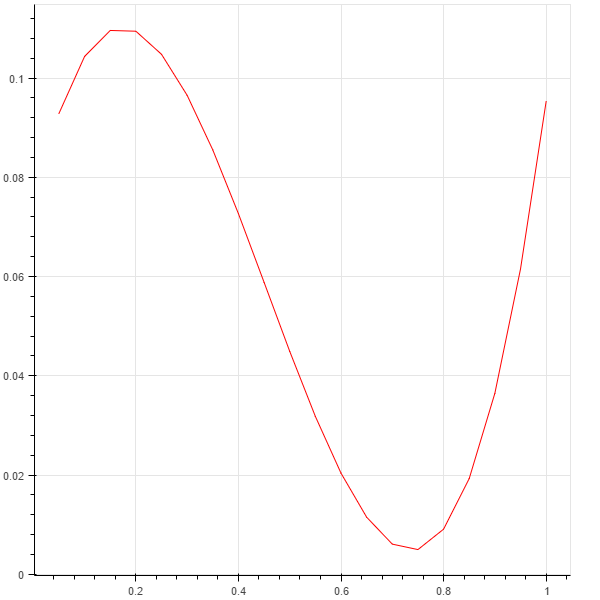
\includegraphics[width=40mm]{RF_analysis/n_100.png}
		\caption{N= 100}
		\label{fig:a} %  
	\end{subfigure}
	\begin{subfigure}[t]{0.3\textwidth}
		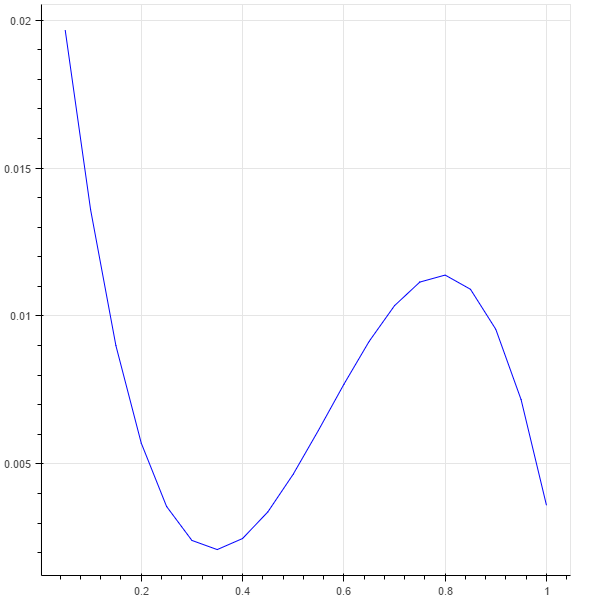
\includegraphics[width=40mm]{RF_analysis/n_1000.png}
		\caption{N = 1000}
		\label{fig:b}
	\end{subfigure}


	\begin{subfigure}[t]{0.3\textwidth}
		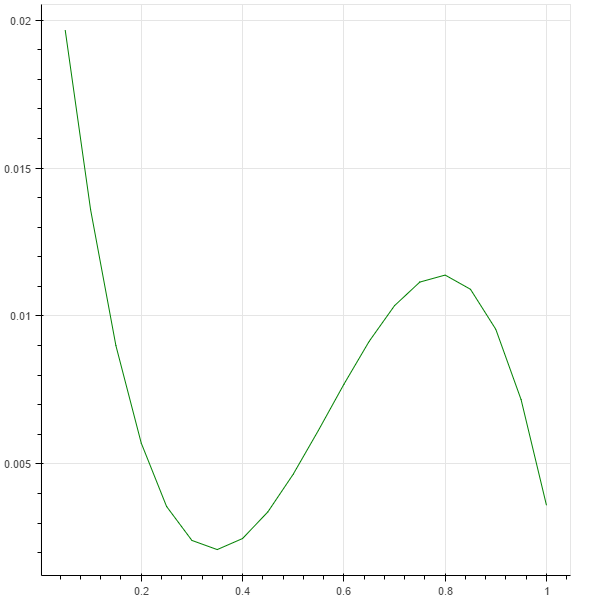
\includegraphics[width=40mm]{RF_analysis/n_10000.png}
		\caption{N = 10.000}
		\label{fig:c}
	\end{subfigure}	
	\begin{subfigure}[t]{0.3\textwidth}
		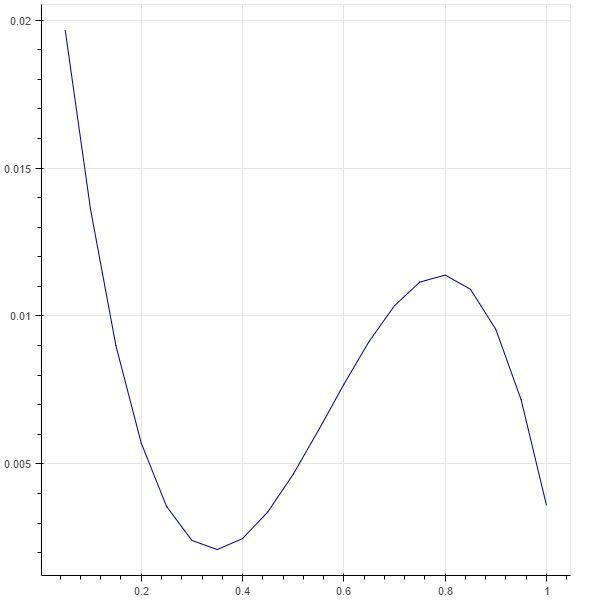
\includegraphics[width=40mm]{RF_analysis/n_50000.png}
		\caption{N = 50.000}
		\label{fig:d}
	\end{subfigure}
\caption{Pricing error with number of maximum leafs for different number of samples N}
\end{figure}

Apart from N=100, the number of maximum leafs seems to be optimal when limited to 30\%-35\% of the samples N.

Higher values must be due to over-fitting, when smaller values are due to under-fitting.
See Appendix B for more details. 



\begin{figure}[H]
	\centering
	\begin{subfigure}[t]{0.3\textwidth}
		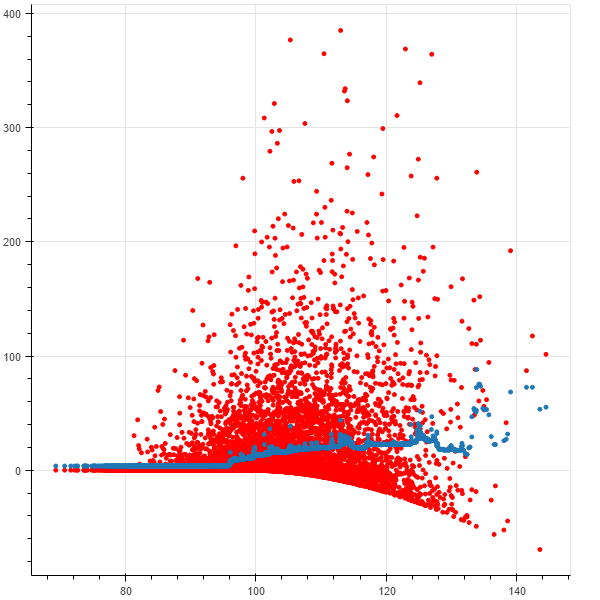
\includegraphics[width=40mm]{RF_analysis/RF_10.png}
		\caption{b=10}
		\label{fig:a} %  
	\end{subfigure}
	\begin{subfigure}[t]{0.3\textwidth}
		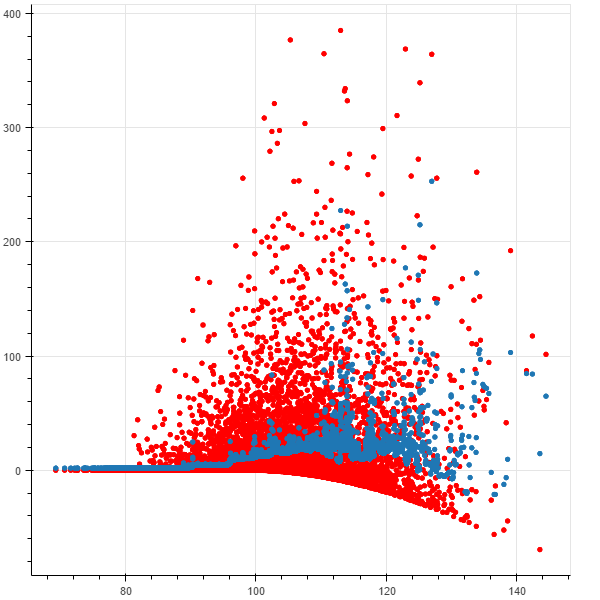
\includegraphics[width=40mm]{RF_analysis/RF_100.png}
		\caption{b=100}
		\label{fig:b}
	\end{subfigure}
	\begin{subfigure}[t]{0.3\textwidth}
		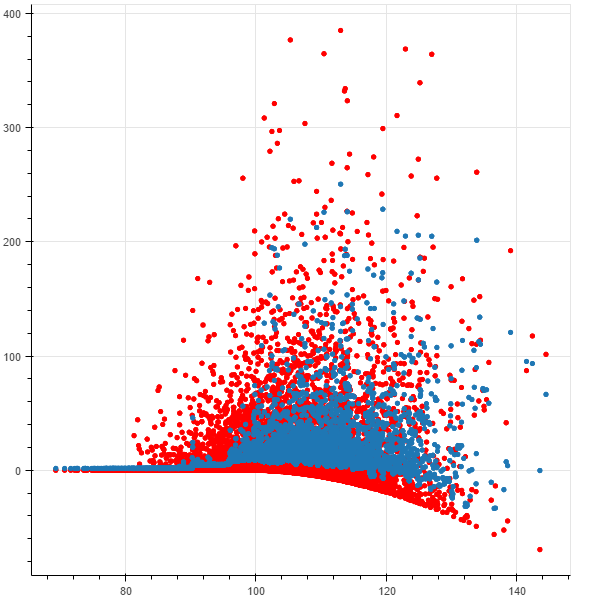
\includegraphics[width=40mm]{RF_analysis/RF_500.png}
		\caption{b=500}
		\label{fig:c}
	\end{subfigure}	
	
	\begin{subfigure}[t]{0.3\textwidth}
		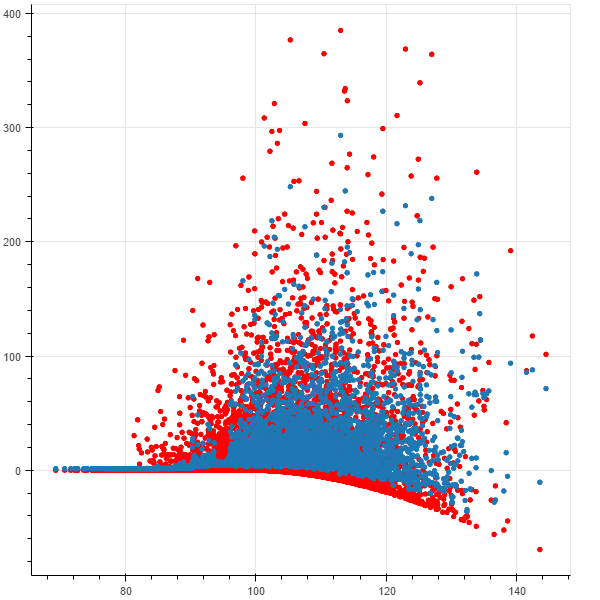
\includegraphics[width=40mm]{RF_analysis/RF_1000.png}
		\caption{b=1000}
		\label{fig:d}
	\end{subfigure}
	\begin{subfigure}[t]{0.3\textwidth}
		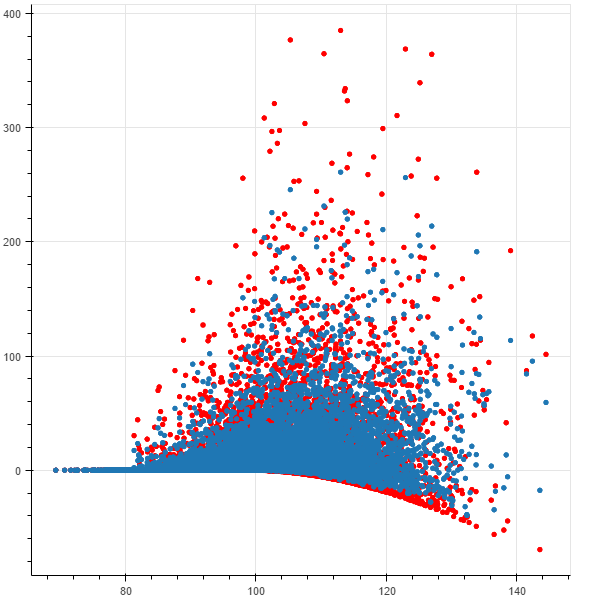
\includegraphics[width=40mm]{RF_analysis/RF_5000.png}
		\caption{b=1000}
		\label{fig:c}
	\end{subfigure}	
	\begin{subfigure}[t]{0.3\textwidth}
		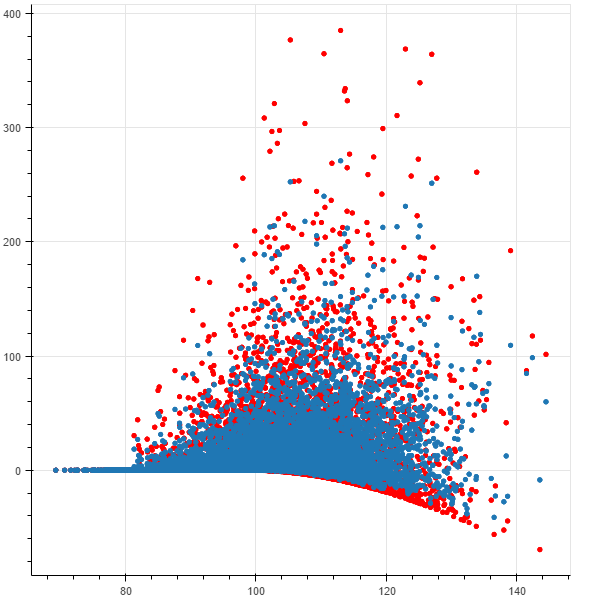
\includegraphics[width=40mm]{RF_analysis/RF_10000.png}
		\caption{b=10000}
		\label{fig:d}
	\end{subfigure}
	
	\caption{Display of the regression step using RF method (in blue) and display of $Y_{t}\frac{\Delta B_t}{\Delta t}$ (red) , both with respect to $X_t$, fixing the number of samples to 10.000 and playing with number of leafs b}
\end{figure}


 \subsubsection{Derivative}

Processing in a first time a Random Forest, we follow the derivative algorithm presented in previous chapter, using kernel regression. 

Let us draw prices computed with respect to scaling parameter l, and samples N.

\begin{table}[H]
	\centering
	\caption{Derivative method with number of paths and scale parameter $l$}
	\label{table:derivative}
	\begin{tabular}{|l|c|c|c|c|c|c|}\hline
		l & N = 100           & N = 500           & N = 1000          & N = 4000          & N = 10000         \\
		\hline
		0.1 &7.54 (1.156)  & 7.26 (0.383)  & 7.245 (0.286) & 7.278 (0.174) & 7.231 (0.102) \\\hline
		0.2 & 6.944 (0.933) & 7.223 (0.376) & 7.224 (0.299) & 7.276 (0.176) & 7.249 (0.118) \\\hline
		0.3 & 7.232 (0.848) & 7.206 (0.425) & 7.284 (0.354) & 7.273 (0.131) & 7.253 (0.103) \\\hline
		0.4 & 7.078 (1.123) & 7.232 (0.469) & 7.307 (0.372) & 7.325 (0.182) & 7.266 (0.114) \\\hline
		0.5 & 6.989 (0.958) & 7.218 (0.491) & 7.243 (0.304) & 7.327 (0.184) & 7.275 (0.123) \\\hline
		1 & 7.257 (1.007) & 7.406 (0.436) & 7.366 (0.271) & 7.241 (0.175) & 7.278 (0.112) \\\hline
		2 & 7.522 (0.932) & 7.37 (0.436)  & 7.387 (0.255) & 7.241 (0.157) & 7.274 (0.097) \\\hline
		5 & 7.149 (0.993) & 7.471 (0.48)  & 7.264 (0.286) & 7.275 (0.169) & 7.316 (0.1)   \\\hline
		10 & 7.509 (0.787) & 7.429 (0.355) & 7.303 (0.264) & 7.353 (0.167) & 7.339 (0.098) \\\hline
		20 & 7.607 (0.972) & 7.312 (0.449) & 7.339 (0.463) & 7.44 (0.167)  & 7.441 (0.095) \\\hline
		50 & 7.126 (0.939) & 7.304 (0.412) & 7.536 (0.345) & 7.456 (0.17)  & 7.462 (0.097) \\\hline
		100 & 7.532 (1.328) & 7.486 (0.456) & 7.46 (0.346)  & 7.488 (0.149) & 7.473 (0.085) \\\hline
		200 & 7.29 (0.754)  & 7.46 (0.492)  & 7.421 (0.227) & 7.468 (0.173) & 7.472 (0.123) \\\hline
		\hline
	\end{tabular}
\end{table}

Despite a smoother process $Z$ and calibration of scaling parameter $l$, results are too far from expectation of 7.15, both biased and with high variance. 

The following figures mostly explain high variances noticed before.

\begin{figure}[H]
	\centering
	\begin{subfigure}[t]{0.3\textwidth}
		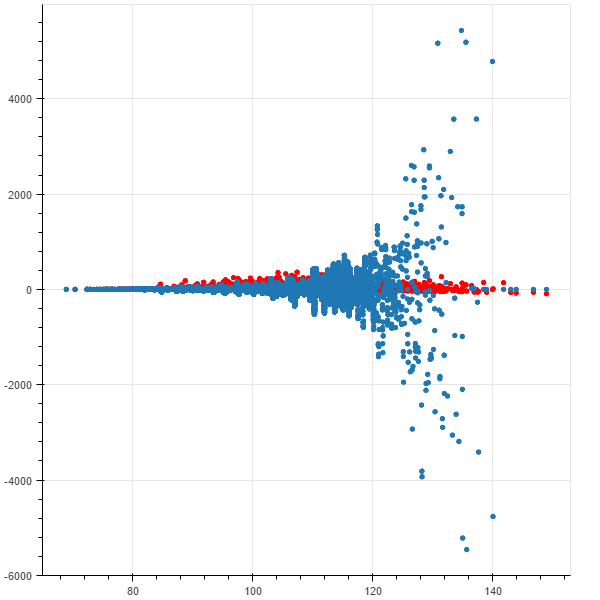
\includegraphics[width=30mm]{kernel_regression/l=01.png}
		\caption{l = 0.1}
		\label{fig:a} %  
	\end{subfigure}
	\begin{subfigure}[t]{0.3\textwidth}
		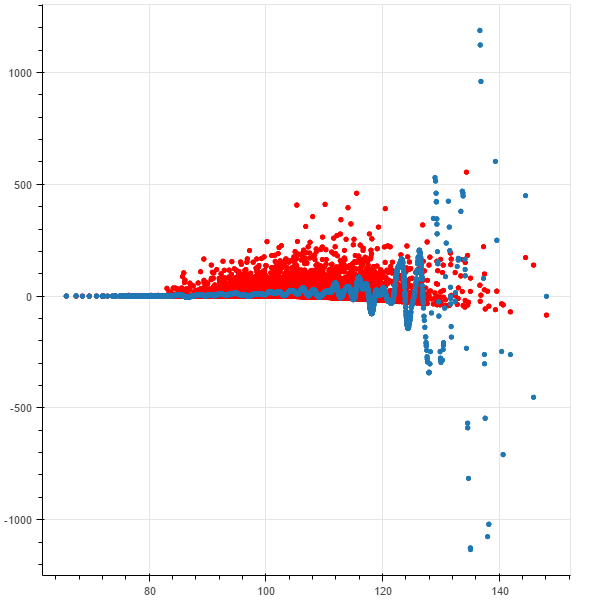
\includegraphics[width=30mm]{kernel_regression/l=05.png}
		\caption{l = 0.5}
		\label{fig:b}
	\end{subfigure}
	\begin{subfigure}[t]{0.3\textwidth}
		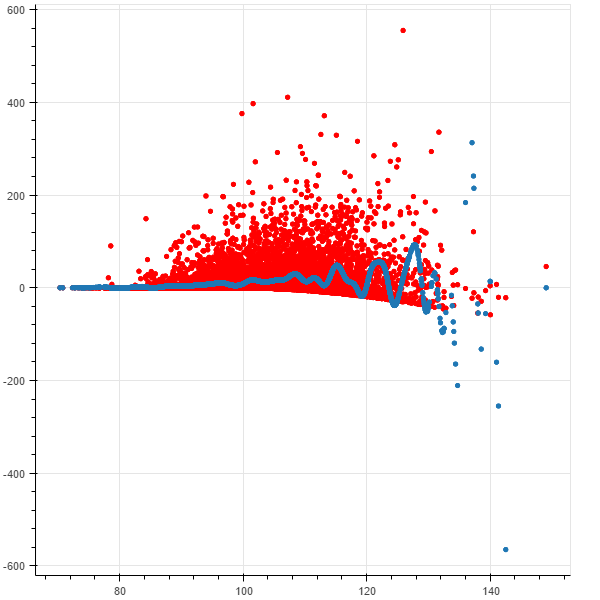
\includegraphics[width=30mm]{kernel_regression/l=1.png}
		\caption{l = 1}
		\label{fig:c}
	\end{subfigure}


	\begin{subfigure}[t]{0.3\textwidth}
		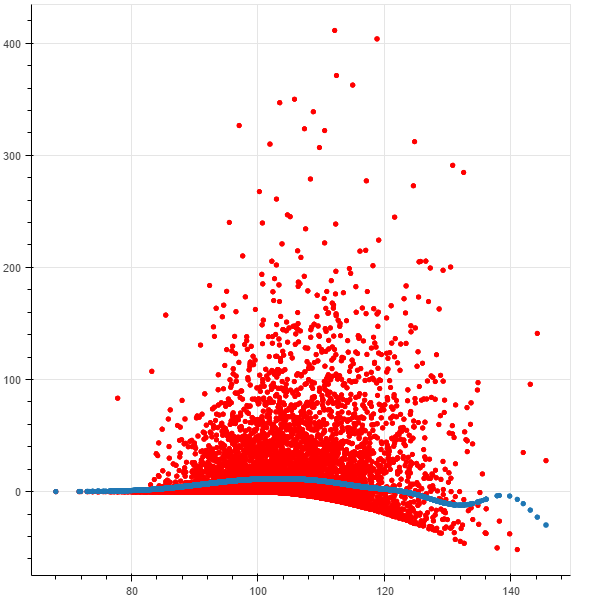
\includegraphics[width=30mm]{kernel_regression/l=5.png}
		\caption{l = 5}
		\label{fig:d}
	\end{subfigure}
	\begin{subfigure}[t]{0.3\textwidth}
		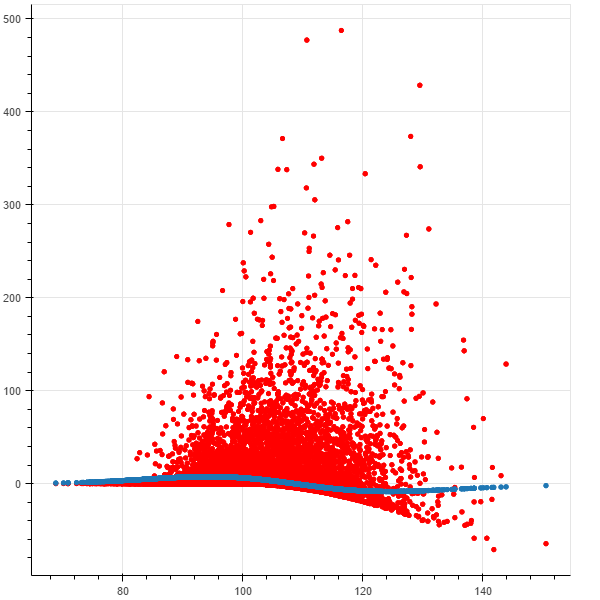
\includegraphics[width=30mm]{kernel_regression/l=10.png}
		\caption{l = 10}
		\label{fig:e}
	\end{subfigure}
	\begin{subfigure}[t]{0.3\textwidth}
		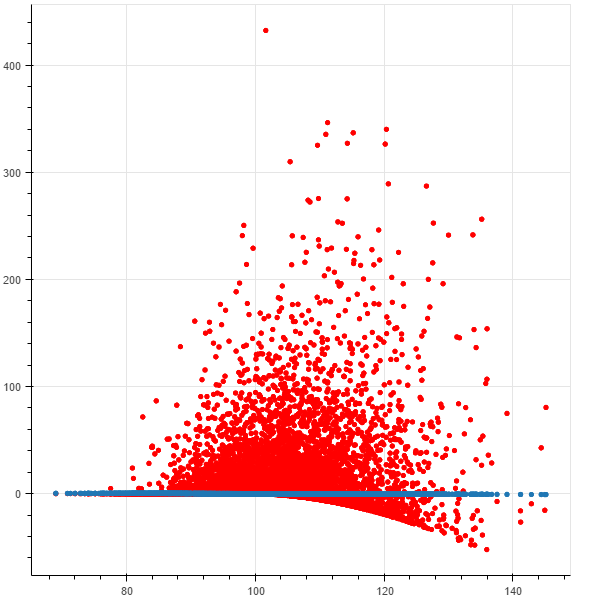
\includegraphics[width=30mm]{kernel_regression/l=100.png}
		\caption{l = 100}
		\label{fig:f}
	\end{subfigure}
\end{figure}

\begin{figure}	
	
\end{figure}

\subsubsection{Summary}
 
Specifically to each method, table \eqref{table:bid_ask_european_call_1D} gives the best calibration, and main statistical measures, with the time average of one run.
Results correspond to the same number of time step, $m=6$.

\begin{table}[H]
	\centering
	\caption{Bid-ask European call option with one asset}\label{table:bid_ask_european_call_1D}
	\rowcolors{5}{}{gray!10}
	\begin{tabular}{*5c}
		\toprule
		& \multicolumn{3}{c}{European Call} \\
		\cmidrule(lr){2-5}
		Method & Random Forest  & Least-Square & Mesh & Derivative \\    
		& $(200, 3000)$ & degree = $6$     &  &  l = 1.0\\
		& N = 10.000 & N = 100.000     & $N = 10 000$  &$N = 4 000$   \\
		\midrule
		mean &     7.142   & 7.155  &  7.152  &  7.231 \\ 
		95\% CI &   $[7.134, 7.150]$     &    $[7.152, 7.159]$     & $[7.117, 7.187]$ & $[7.191, 7.271]$  \\
		time average &  35s   & 5s & 30s & 4s \\
		\bottomrule
	\end{tabular}
\end{table}

\begin{Rem}
	C.I stand for confidence interval, while (200, 3000) corresponds to number of trees generated and maximum number of leafs allowed respectively.
\end{Rem}

\begin{Rem}
	Random Forest performs well in accuracy, but time computation is high compared to the other methods. However, with higher dimensions, this method will prove efficient...
\end{Rem}

\begin{Rem}
For the following applications, an equivalent table to \ref{table:bid_ask_european_call_1D} will be given only.
However, the same calibrations have been run to obtain the best hyper-parameters.
\end{Rem}


\subsection{Bid-ask European call combination}

Once again, we take an example from Gobet, Lemor and Warin's 's article \cite{gobet:example}, where we consider still two different rates (bid-ask model). This time, the differences $R-r$ and $\mu - r$ are larger, as $\mu = 0.05$, $r=0.01$ and $R=0.06$. This emphasizes the role of the noisy process $Z$ during the regression steps. 
We keep working with a 20\% volatility $\sigma=0.02$, no dividend yield $q=0$, and an initial asset value $X_0 = 100$. We consider a call combination derivative, with pay-off $(X_T - K_1)^+ - 2(X_T - K_2)^+$, where $K_1 = 95$ and $K_2 = 105$.

In their simulations, Gobet, Lemor and Warin's use projections on function basis to approximate the conditional expectations. They make use of hypercubes partitions, Voronoi partitions (VP) and global polynomials.

There is no theoretical price for this example, as the non-linearity of driver has a real impact. The option buyer has alternatively to borrow and lend money to hedge his position.

However, a simulation price given by Hypercubes and VP seem to converge to 2.95, which will be taken as reference. 
Applying our derivative, stochastic mesh, LSM and Random Forest methods to this example, we get

\begin{table}[H]
	\centering
	\caption{Bid-ask European call combination option with one asset}\label{table:bid_ask_call_combi_1D}
	\rowcolors{5}{}{gray!10}
	\begin{tabular}{*5c}
		\toprule
		& \multicolumn{3}{c}{Call combination } \\
		\cmidrule(lr){2-5}
		Method & Random Forest  & Least-Square & Mesh & Derivative \\    
		& $(200, 3000)$ & degree = $6$     &  & l= 1.0\\
		& N = 10.000 & N = 100.000     & $N = 10 000$ &  $N = 4 000$   \\
		\midrule
		mean &     2.969   & 2.938  &  2.921  &  2.940 \\ 
		95\% C.I &   $[2.965, 2.974]$     &    $[2.937, 2.940]$     & $[2.904, 2.938]$ & $[2.912, 2.969]$  \\
		time average &  45s      & 5s  & 30s & 9s \\
		\bottomrule
	\end{tabular}
\end{table}

\begin{Rem}
	
\end{Rem}

\subsection{CVA}

Following Guyon and Labordère example \cite{GuyonLabordere:cva}, i.e with $X_0 = 1.$, $\sigma = 0.2$, $\mu=r=0.$, $g:x \rightarrow 1 - 2.\mathbbm{1}_{x>1}$ (final condition) and $\beta = 10\%$

\begin{table}[H]
	\centering
	\caption{CVA via BSDE compared to Guyon and Labordère PDE method}\label{table:CVA}
		\begin{tabular}{|l|c|c|}\hline
			Maturity (years) & PDE with poly & Random Forest (std) \\ \hline
			2      &  11.62 &   11.663(0.011)   \\ \hline
			4     &  16.54 &    16.613 (0.009)    \\ \hline
			6   & 20.28  &   20.595(0.010)   \\  \hline
			8  &  23.39 &   23.587(0.012)  \\  \hline
			10  &  26.11 &   26.107 (0.009)   \\  \hline
	\end{tabular}
\end{table}

\begin{Rem}
	We train 150 trees on $N = 10.000$ particles generated, and to avoid overfitting, we limit the depth of trees to $1000$ leafs, i.e $10\%$ of the samples. Time average for a run is around 6s. 
\end{Rem}


\subsection{American Call Option}

We consider an American maximum call option with ten exercising 

\begin{table}[H]
	\centering
	\begin{tabular}{ |l|c|c|c|c|c|c|}\hline
		r & $\sigma$ & q & T  & K   & $X_0$    \\ \hline
		0.05   & 0.2  & 0.1 & 3 & 100 & 100      \\ \hline
		
	\end{tabular}
\end{table}

with final pay-off $Y_T = \left(X_T -K\right)^+$. 
We take the results by Glasserman (2004) \cite{glasserman:amoption} as a comparison, who get a price of 7.98 using a binomial lattice. 

\begin{table}[H]
	\centering
	\caption{Call combination of geometric average }\label{table:am_option}
	\rowcolors{5}{}{gray!10}
	\begin{tabular}{*3c}
		\toprule
		& \multicolumn{2}{c}{Methods tested} \\
		\cmidrule(lr){2-3}
		Method  & LSM & Random Forest \\    
		& $N = 100.000$ & $(200, 850)$    \\
		 &  & $N = 10.000$    \\
		\midrule
		mean & 7.977  &   7.990     \\ 
		95\% C.I & [7.974, 7.988] &  [7.938, 8.041]     \\
		time average &   2s     &  20s
		\\
		\bottomrule
	\end{tabular}
\end{table}

\section{High Dimension}

\subsection{Geometrical average on seven assets following bid-ask model}

After managing to tune our Random Forest hyperparameters in one dimension cases, we now turn to more sophisticated problems. 
First case which drew our attention is the pricing of a Geometrical Average call option on seven assets. This derivative has a payoff $((\prod_{i=1}^{7}X_T^{(i)})^{\frac{1}{7}} - K)^+$. 
Taking seven independent assets in Black-Scholes model, this problem is equivalent to taking a one dimensional European call. 

Indeed, let us assume $\forall i \in \{1, \cdots, d\}$, $X_T^{i} = X_0^{i} \exp^{(r - \frac{\sigma^2}{2})T + \sigma B_T^{i}}$. 
Then 

\begin{align}
(\prod_{i=1}^{7}X_T^{(i)})^{\frac{1}{d}} &= X_0 \exp^{(r - \frac{\sigma^2}{2})T + \frac{\sigma}{d}\sum_{i=1}^{d}B_T^{i}} \notag \\
&\overset{\mathcal{L}}{\sim} X_0 \exp^{(r - \frac{\sigma^2}{2})T + \frac{\sigma}{d}\sum_{i=1}^{d}\mathcal{N}(0, T)} \notag \\
&\overset{\mathcal{L}}{\sim} X_0 \exp^{(r - \frac{\sigma^2}{2})T + \frac{\sigma}{d}\mathcal{N}(0, dT)} \notag \\
&\overset{\mathcal{L}}{\sim} X_0 \exp^{(r - \frac{\sigma^2}{2})T + \frac{\sigma}{\sqrt{d}}\mathcal{N}(0, T)} \notag
\end{align}

Taking 

\begin{align}
 \tilde{r} - \frac{\tilde{\sigma}^2}{2} = r - \frac{\sigma^2}{2} \\
\tilde{\sigma} = \frac{\sigma}{\sqrt{d}}
\end{align}

\begin{align}
\tilde{r} = r + \frac{\sigma^2}{2}\frac{d-1}{d} \\
\tilde{\sigma} = \frac{\sigma}{\sqrt{d}}
\end{align}

\begin{displaymath}
(\prod_{i=1}^{7}X_T^{(i)})^{\frac{1}{d}} \overset{\mathcal{L}}{\sim} X_0 \exp^{(\tilde{r} - \frac{\tilde{\sigma}^2}{2})T + \tilde{\sigma}\mathcal{N}(0, T)}
\end{displaymath}

Hence, a theoretical price is given by usual Black-Scholes formula 
\begin{displaymath}
 Y_0 = BS(T, K, X_0, \tilde{r}, \tilde{\sigma}) = 3.308
\end{displaymath}
where  $X_0 = 100 \mathbbm{1}_d$ ($\mathbbm{1}_d$ being the unit vector with $d$ ones), $K=100.$, $\sigma=0.2Id$, $r=0.04$, $R=0.06$, $\mu = 0.06\mathbbm{1}_d$ and $q = 0$. 

\subsubsection{Random Forest Analysis}

\begin{table}[H]
	\centering
	
	\begin{tabular}{|l|c|c|c|c|c|c|}\hline
		K & b= 200   & b = 500 & b = 1000  & b = 1500   & b=2000    \\ \hline
		1   & 3.29 (0.034)  & 3.256 (0.035) & 3.238 (0.032) & 3.274 (0.037) & 3.272 (0.039)       \\ \hline
		2   & 3.286 (0.038) & 3.25 (0.029)  & 3.279 (0.032) & 3.294 (0.032) & 3.317 (0.028)   \\ \hline
		3     & 3.266 (0.033) & 3.256 (0.033) & 3.293 (0.038) & 3.327 (0.033) & 3.345 (0.029)  \\ \hline
		4  & 3.278 (0.044) & 3.266 (0.03)  & 3.297 (0.035) & 3.336 (0.028) & 3.359 (0.032) \\ \hline
		5  & 3.263 (0.039) & 3.272 (0.038) & 3.317 (0.035) & 3.344 (0.042) & 3.375 (0.027)  \\  \hline
		6 & 3.273 (0.04)  & 3.267 (0.037) & 3.32 (0.041)  & 3.357 (0.043) & 3.38 (0.05)   \\\hline
		7 & 3.257 (0.034) & 3.289 (0.041) & 3.32 (0.041)  & 3.34 (0.037)  & 3.369 (0.036) \\\hline
		\hline
		
	\end{tabular}
\caption{Random Forest with maximum number of features K and maximum number of leafs b}
\label{table:high_dim_rf_feat_leafs}
\end{table}

Given the uncorrelated assets, number of features does not seem to affect so much the pricing. However it seems to affect the number of leafs to calibrate. 
Literature \cite{glouppe:rf} advices an optimal number of features $K=\frac{d}{3}$ to take when running a Random Forest.  

\begin{table}[H]
	\centering
	
	\begin{tabular}{|l|c|c|c|c|c|c|}\hline
		K & b= 200   & b = 500 & b = 1000  & b = 1500   & b=2000    \\ \hline
		1 & 75.03 &  75.28 &  78.15 &  80.18 &  83.77 \\ \hline
		2 & 73.88 &  77.22 &  98.62 &  91.44 &  94.14 \\ \hline
	3 & 	83.18 &  87.33 &  89.55 &  94.38 &  95.73 \\ \hline
	4 & 	82.91 &  87.58 &  92.49 &  94.46 & 100.41 \\ \hline
	5 & 	83.5  &  90.26 &  96.04 & 102.63 & 106.44 \\ \hline
	6 & 	86.12 &  93.37 & 102.63 & 122.22 & 112.97 \\ \hline
	7 & 	89.46 & 100.47 & 109.51 & 115.49 & 119.11 \\ \hline
		\hline
	\end{tabular}
	\caption{Random Forest time computation with dimension d and maximum number of leafs in seconds \label{table:high_dim_time}}
\end{table}

\subsubsection{Results}

\begin{table}[H]
	\centering
	\caption{Bid-ask  Geometric Average European Call option on 7 assets}\label{table:call7D}
	\rowcolors{5}{}{gray!10}
	\begin{tabular}{*4c}
		\toprule
		& \multicolumn{3}{c}{Geometric Average European Call} \\
	Method & Random Forest   & Mesh & Derivative \\  
	
	& $(200, 700)$ &    &  l = 1.0 \\
	& N = 10.000 & N = 10.000      &   $N = 4 000$\\
	\midrule
	mean &     3.299   &  3.318  &  3.330 \\ 
	95\% confidence interval &   $[3.296, 3.304]$   & $[3.310, 3.327]$ & $[3.260, 3.401]$  \\
	time average &    1min10s  & 2min20s & 40s \\
		\bottomrule
	\end{tabular}
\end{table}


\begin{Rem}
	Even if Derivative method performs better in matter of time, its variance is too high compared to Random Forest one. 
	Mesh method performs well in term of accuracy, but time computation does not challenge Random Forest 
\end{Rem}

\begin{Rem}
	For Mesh in high dimension, density functions can be expressed as the product of one-dimensional densities.
\end{Rem}

\begin{comment}
\subsection{Geometrical average on twenty-five assets following bid-ask European call model}

\begin{table}[H]
	\centering
	\caption{Bid-ask European call option with one asset}\label{table:1}
	\rowcolors{5}{}{gray!10}
	\begin{tabular}{*5c}
		\toprule
		& \multicolumn{3}{c}{Methods tested} \\
		\cmidrule(lr){2-4}
		Method & Random Forest  & Least-Square & Mesh & Derivative \\    
		& $(200, 700)$ & degree = $6$     & $N = 4 000$ &  $N = 4 000$ \\
		\midrule
		mean &     7.142   &  &       \\ 
		95\% confidence interval &        &        & CHECK \\
		time average &        & CHECK & CHECK \\
		\bottomrule
	\end{tabular}
\end{table}

\end{comment}

\subsection{Geometrical average on twenty assets following bid-ask European call combination model}

Expected 5.70, using the equivalent problem of a call combination on one asset. As this problem does not have a theoretical value, and literature does not offer comparison, we take the result obtained by Random Forest ran on 100.000 samples (which was the most reliable method in one dimension). 

\begin{table}[H]
	\centering
	\caption{Call combination of geometric average }\label{table:1}
	\rowcolors{5}{}{gray!10}
	\begin{tabular}{*5c}
		\toprule
		& \multicolumn{3}{c}{Methods tested} \\
		\cmidrule(lr){2-4}
		Method & Random Forest & Mesh & Derivative \\    
		& $(200, 700)$    & & $l=1.$  \\
		& $N = 10.000$    &  $N = 4 000$ &  $N = 4 000$  \\
		\midrule
		mean &     5.686    &  5.688 &  5.6694  \\ 
		95\% confidence interval &  [5.675, 5.697]      &  [5.684, 5.693]      & [5.691, 5.708]  \\
		time average &   1min52s     &  5min48s & 3min \\
		\bottomrule
	\end{tabular}
\end{table}

\begin{Rem}
	We limited every tree generated to four features chosen randomly, which allowed a faster computation than mesh, and with more samples !
	We can notice a good estimation provided by derivative method when dimension is higher.
\end{Rem}

\subsection{Max Call Option on 5 assets}

We consider an American maximum call option with ten exercising 

\begin{table}[H]
	\centering
	\begin{tabular}{ |l|c|c|c|c|c|c|}\hline
		r & $\sigma$ & q & T  & K   & $X_0$    \\ \hline
		0.05   & 0.2  & 0.05 & 3 & 100 & 100      \\ \hline
		
	\end{tabular}
\end{table}

with final pay-off $Y_T = \left(\underset{i}{max}X_T^{(i)} -K\right)^+$. 
We take the results by Broadie and Glasserman (2004) \cite{broadie2004stochastic} as a comparison, who get a price of 23.052 using stochastic mesh. 

\begin{table}[H]
	\centering

	\rowcolors{5}{}{gray!10}
	\begin{tabular}{*5c}
		\toprule
		& \multicolumn{3}{c}{Methods tested} \\
		\cmidrule(lr){2-4}
		Method & Random Forest & Mesh & Derivative \\    
		& $N = 10.000$    & $N = 4 000$ &  $N = 4 000$ \\
		&   $(200, 700)$  &  &  $l=1.$ \\
		\midrule
		mean &     23.016   &  22.949 &  22.913  \\ 
		95\% confidence interval &  [22.988, 23.044]      &  [22.905, 22.992]      & [22.844, 22.982]  \\
		time average &   20s     &  29s & 14s \\
		\bottomrule
	\end{tabular}
	\caption{Max Call option on 5 assets }\label{table:1}
\end{table}

\begin{Rem}
	This 5 dimensional problem has a linear driver, thus a low computation obtained. However, Mesh and derivative seem far from price provided by Glasserman. 
\end{Rem}

\subsection{Exchange Option between two correlated assets}

We consider in this model two correlated assets $X^{(1)}$ and $X^{(2)}$ to define an exchange pay-off $\xi(X^{(1)}_T, X^{(2)}_T) = \left(X^{(1)}_T - X^{(2)}_T\right)^+$. 
This 2-dimensional problem is really interesting, as it has a theoretical solution, and is going to test how Random Forest performs here when there is correlation.
 This theoretical solution , called Margrabe Formula is given by Poulsen and Rolf in \cite{poulsen2009margrabe}. 
Let us assume that the interest rate is constant (r) and that the underlying assets follow correlated ($\langle dB^{(1)}_t, dB^{(2)}_t \rangle =\rho dt$) geometric Brownian motions under the risk-neutral measure. 

Time t-value $Y_t = u(t, X^{(1)}_t, X^{(2)}_t)$ of this exchange option is

\begin{displaymath}
Y_t = X^{(1)}_t \exp^{(\mu_1 - r)(T-t)}\Phi(d_+) - X^{(2)}_t \exp^{(\mu_2 - r)(T-t)}\Phi(d_-)
\end{displaymath}

where 

\begin{displaymath}
d_{\pm} = \frac{\ln\left(\frac{X^{(1)}_t}{X^{(2)}_t}\right) + (\mu_1 - \mu_2 \pm \frac{\tilde{\sigma}^2}{2} ) }{\tilde{\sigma}\sqrt{T-t}}
\end{displaymath}

and 

\begin{displaymath}
\tilde{\sigma} = \sqrt{\sigma_1^2  + \sigma_2^2 - 2\sigma_1\sigma_2 \rho}
\end{displaymath}

\begin{table}[H]
	\centering
	\caption{Bid-ask European call option with one asset}\label{table:eo}
	\rowcolors{5}{}{gray!10}
	\begin{tabular}{*5c}
		\toprule
		& \multicolumn{3}{c}{Random Forest (Trees, Max\_leafs)} \\
		\cmidrule(lr){2-4}
		 & $(200, 1000)$ &  $(200, 2000)$ & $(200, 3000)$ \\
		\midrule
		mean &      4.077 &    4.128   & 4.181\\ 
		95\% confidence interval &  [4.044, 4.091]    & [4.109, 4.147] & [4.163, 4.199] \\
		average time &   55s & 60s & 65s \\
		\bottomrule
	\end{tabular}
\end{table}

\begin{Rem}
Random Forest performs well with limitation to 20\% of leafs for these two correlated assets problem. 
Hence the importance of prior calibration when using this method. 

We do not run a mesh for this example as density function for such correlated paths does not exist analytically.
\end{Rem}

\subsection{Exchange Option between the average of twenty correlated assets}

We analyse in this case an equivalent of previous exchange option, but with twety correlated assets. The pay-off $\xi(X^{(1)}_T, \cdots ,X^{(20)}_T) = \left(\prod_{i=1}^{10}X^{(i)}_T - \prod_{i=11}^{20}X^{(i)}_T\right)^+$. 
For the rest, the parameters are equivalent to previous case.

\begin{table}[H]
	\centering
	\caption{Bid-ask European call option with one asset}\label{table:eo20}
	\rowcolors{5}{}{gray!10}
	\begin{tabular}{*5c}
		\toprule
		& \multicolumn{3}{c}{Random Forest (Trees, Max\_features)} \\
		\cmidrule(lr){2-4}
		& $(200, 1)$ &  $(200, 3)$ & $(200, 6)$  & (200, 10)\\
		\midrule
		mean &      1.395  &    1.351  & 1.360 & 1.362\\ 
		95\% CIl &  [1.367, 1.411]  &  [1.347, 1.357] & [1.357, 1.363] & [1.361, 1.363] \\
		average time &   1mn10s & 2mn11s & 3mn30s & 5mn \\
		\bottomrule
	\end{tabular}
\end{table}
 

A theoretical price can be derived like using previous formula with equivalent $\rho$ and $\sigma_1$, $\sigma_2$ especially. This formula gives an equivalent price of 1.356, which compares well to simulations with more than 3 features. 

\chapter{Second Order BSDE}

This section presents an extension to 1-BSDE models, with a direct application on non-linear PDE.
Cheridito, Soner, Touzi and Victoir \cite{cheridito:2BSDE} introduced the notion of Second Order BSDEs (2-BSDEs).
\newline
We will give a quick definition of the problem, before explaining the link with non-linear PDE. We will finish with an example of discretization for this type of BSDE. 
For a larger review of the theory of 2-BSDEs, we refer to Soner, Touzi and Zhang \cite{touzi:2BSDE}.

\section{Definition}

We now introduce second
order BSDEs for which the corresponding PDE can be non-linear in the second
order derivatives and are therefore connected to HJB equations with a control on the diffusion coefficient. Examples of such HJB equations include the
Black-Scholes-Barenblatt equation.
The following definition is given by \cite{cheridito:2BSDE}

\begin{defn}
Let $(s, x) \in \left[0, T\right) \times\R^d$ and $(Y_t, Z_t, \Gamma_t, \alpha_t)_{t\in [0, T]}$ be a quadruple of $(\mathcal{F}_t)$-adapted processes taking values in $\R$, $\R^d$, $\mathcal{S}^d$ \footnote{Space of symmetrical matrices with dimension}, and $\R^d$ respectively. We call $(Y, Z, \Gamma, \alpha)$ a solution to a 2-BSDE corresponding to $(X^{s,x}, f, g)$ \footnote{$X_s = x$} if
	
\begin{align} \label{2-BSDE}
dY_t &= - f(t,X_t^{s,x}, Y_t,Z_t, \Gamma_t)dt + Z_t' \diamond dX_t^{s,x} \quad t\in [s, T)\\
dZ_t &= \alpha_tdt + \Gamma_t dX_t^{s,x} \quad t\in [s, T) \notag\\
Y_T & = g(X_T^{s,x}) \notag
\end{align}
where $\diamond$ represents the Stratanovich integral, related to Itô integration by 

\begin{align}
Z_t' \diamond dX_t^{s,x} &= Z_t' dX_t^{s,x} + \frac{1}{2}d\langle Z, X_t^{s,x}\rangle_t \notag \\
&= Z_t' dX_t^{s,x} + \frac{1}{2}Tr\left[\Gamma_t d\langle X_t^{s,x}, X_t^{s,x}\rangle_t \right] \notag \\
& = Z_t' dX_t^{s,x} + \frac{1}{2}Tr\left[\Gamma_t \sigma(t, X_t^{s,x})\sigma(t, X_t^{s,x})' \right]dt \notag
\end{align}

\end{defn}

\section{Existence and Uniqueness}

The reader can refer to "Wellposedness of Second Order Backward SDEs" \cite{touzi:2BSDE} article which provides an existence and uniqueness theory. 

\section{Second order BSDE and non-linear PDE}

Let us consider the non-linear PDE 
\begin{equation}\label{eq:nonlinearpde}
\partial_t u + \mathcal{L}u + f(t, x, u, D_xu(t,x), D^2_xu(t,x)) = 0, \quad (t,x)\in [0, T) \times \mathbb{R}^d
\end{equation}
with the terminal condition $u(T; x) = g(x)$ and $\mathcal{L}$ the Itô generator of $X$.
Such an equation appears when we consider a stochastic control problem
with no control on the diffusion coefficient. 
($Y_t = u(t;X_t)$ , $Z_t =D_xu(t;X_t)$, $\Gamma_t = D^2_xu(t;X_t)$, $\alpha_t = (\partial_t + \mathcal{L})D_xu(t,X_t)$) is a solution to the 2-BSDE under some assumptions

\begin{Prop}
	Generalization of Feynman-Kac's formula : \newline
	Let $u$ be a function of $\mathcal{C}^{1,2}$ satisfying (\ref{eq:nonlinearpde}) and suppose that there exists a
	constant $C$ such that, for each $(t; x) \in [0; T] \times \mathbb{R}^d$
	\begin{equation}
	|\sigma(t,x)^T D_xu(t;X_t)|\leq C(1 + |x|)
	\end{equation}
	Then $(Y_t = u(t;X_t);Z_t = D_xu(t;X_t), \Gamma_t = D^2_xu(t,x))$ is the unique solution to 2-
	BSDE (\ref{2-BSDE}).
\end{Prop} 


\section{Discretization}

Using the previous tricks (multiplying by $dB_t$ in $dZ_t$ expressions and using measurability properties) gives us the following discretization for the 2-BSDE : 

\begin{align}
Y_{t_n} &= g(X_{t_n}) \notag \\
Z_{t_n} &= Dg(X_{t_n}) \notag \\
\Gamma_{t_i} &= \frac{1}{\Delta t_i}\mathbb{E}[Z_{t_{i + 1}} \Delta B_{t_i}^T  | \mathcal{F}_{t_i}]\sigma(t_i, X_{t_i})^{-1} \notag \\
Z_{t_i} &= \sigma(t_i, X_{t_i})'^{-1}\frac{1}{\Delta t_i}\mathbb{E}[Y_{t_{i + 1}} \Delta B_{t_i}  | \mathcal{F}_{t_i}] \notag 
\end{align}


	
	\begin{displaymath}
	Y_{t_i} = \mathbb{E}[Y_{t_{i + 1}} | \mathcal{F}_{t_i}] +  (f(t_i,S_{t_i}, Y_{t_{i + 1}}, Z_{t_i}, \Gamma_{t_i}) - \mathtt{tr}[\sigma(t_i, X_{t_i}) \sigma(t_i, X_{t_i})'\Gamma_{t_i}])\Delta t_i
	\end{displaymath}


Given $Y_{t_n}$ we can get $Y_0$ using the previous discretization backwardly. 

\section{Application : Portfolio Optimization}

Arash Fahim, Nizar Touzi and Xavier Warin analysed an example of 2-BSDE, the continuous-time portfolio optimization in financial mathematics (\cite{touzi:2bsdesimulation}). 
Two dimensional and Five dimensional examples are solved via non-linear PDE. We tried to solve the problems using 2-BSDE method presented previously, but results obtained do not match exactly the author's one. The reader can refer to the code we released on github  (\textit{https://github.com/MajdiRabia/BSDE.git}) to help fixing it, as second derivative $\Gamma$ can be approximated well using Random Forest regression.

\newpage 


\chapter{Conclusion}

After reviewing BSDE's theory, we gave here several regression methods to compute conditional expectatiosn appearing in the backward algorithm. 
Relying on existent methods found in literature, such as Stochastic Mesh by Broadie and Glasserman \cite{glasserman:broadie} and Least Square \cite{bender:lsmbsde}, we computed different approaches, Random Forest, Gradient, and Derivative, for comparison purposes.
We focused on accuracy (i.e mean and variance), and time analysis to draw simulation conclusions. 


In one dimension, fastest method remains LSM, with promising accuracy when calibrated with a polynomial of degree 6. Random Forest performs well in accuracy terms but drawing several trees slows down the process. Derivative method, even after scale parameter tuning, does not offer reliable results, and even if it was accurate enough, computing $N\times N$ matrices costs time. Mesh method applied with amount of samples costs time but provides a good accuracy. 
Differentiating these methods happens when considering higher dimensions. 


In Higher dimension, Random Forest flexibility to choose a certain amount of features for each tree generated, and calibrated with certain percentage of maximum leafs, gives a really good accuracy and computational time. 

However, this tree based method requires several steps of calibration, and when no theoretical solution exists, or no bounds can be give, it remains difficult to use.



\chapter{Future Work}

Mostly computational, this MSc thesis reviews most numerical methods to solve BSDEs, adding a machine learning method (Random Forest) to price higher dimensional options. 
Given the efficiency of high dimensional pricing with Random Forest, both in accuracy and time computation, compared to stochastic mesh especially, one can now focus on a better calibration method. 

Indeed, had it not been for theoretical solution to our examples, or comparisons in literature, tuning the Random Forest parameters would have been trickier. Depth of trees, number of features, number of leafs are all sensitive parameters. 

We suggest then to the reader some ideas that could be tried, using the code we created and released on github(\textit{https://github.com/MajdiRabia/BSDE.git}). 

First, 'RandomizedsearchCV' and 'RandomizedsearchCV' are two cross-validation methods existing on scikit-learn package with Python.
These two methods could be used during regression step, to calibrate the best hyper-parameters itself. Though it would be timely consuming, it would prove efficient when no theroy exists for a pricing derivative !

Second, reader can improve the existing code for the implemented 2-BSDE computation. 
The current code is only adapted to examples from Warin, Touzi and Fahim \cite{touzi:2BSDE} .If a generic code could be implemented would prove powerful to solve any kind of non-linear PDE, as long as it respects initial conditions.

\newpage
\begin{appendices}
%	
%	\chapter{Model Assessment and Selection}
%	
%	Inspired by Hastie, Tibshirani and Friedman \cite{Friedman:2008}, we present and describe variables used for regression model accuracy measurements.  
%	These key methods enabled the comparisons made during financial applications in part 4. 
%	
%	\section{Bias, Variance and Loss Mean Squared function}
%	
%	
%	\begin{defn} Bias
%		
%		Let $\hat{\mu}$ be an estimator for $\mu = \E[X]$ where $X$ is an integrable random variable. 
%		$\hat{\mu}$ is a an unbiased estimator if $\E[\hat{\mu}] = \mu$. 
%		Inversely, $\mu$ is a biased estimator if the difference between $\E[\hat{\mu}]$ and $\mu$ is not zero. 
%	\end{defn}
%	
%	\begin{defn}Variance
%		
%		Variance is the amount that the estimate of the target function will change if different training data was used.
%		$Var(\hat{\mu}) = \E[\hat{\mu}^2] - \E[\hat{\mu}]^2$
%	\end{defn}
%	
%	Given a target variable $Y$, features $X = (X_1, \cdots, X_p$) and a regression model $\hat{f}$, estimated from a sample set $\mathcal{S}$, we denote $\mathcal{L}$ the loss mean squared function, measuring prediction errors between $Y$ and $\hat{f}(X)$, and defined by 
%	
%	\begin{displaymath}
%	\mathcal{L}(Y, \hat{f}(X)) = ||Y - \hat{f}(X)||^2
%	\end{displaymath}
%	
%	\section{Bias-Variance trade-off}
%	
%	In statistics, bias-variance is the dilemma consisting on reducing simultaneously  two sources of error, bias and variance. 
%	
%	When interested on the expected value of mean squared loss function, one is faced to generalized problem of $\E[(\mu - \hat{\mu})^2]$, i.e
%	
%	\begin{align}
%	\E[(\mu - \hat{\mu})^2] &= \E[(\mu - \E[\hat{\mu}] +  \E[\hat{\mu}] -\hat{\mu})^2] \notag \\
%	& = Bias^2(\hat{\mu}) + Var(\hat{\mu}) + Var(\mu) \notag 
%	\end{align}
%	
%	Most famous Bias-variance trade-off appears in Ridge and Lasso regression models. 
%	When one wants to decrease variance of the model, bias will increase. 
%	The bias-variance decomposition framework can be used as a tool for diagnosing under-fitting % and over-fitting. 
	
\chapter{Random Forest}

\section{Complexity}

Let us consider p predictor variables $(x_1, \cdots, x_p) \in D \subset \R^p$  of a response variable $y$. The goal of this subsection is to determine the time complexity of the Random Forest model, given $N$ samples data. 
\newline
Let $T(N)$ denote the time for building one decision tree. 

\begin{figure}[h!]
	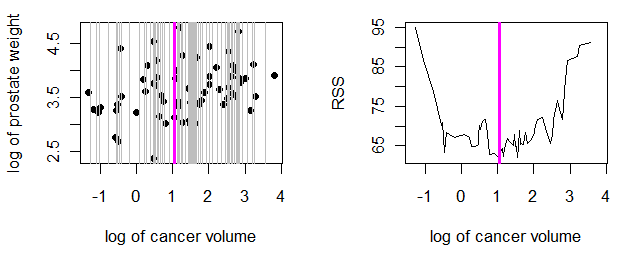
\includegraphics[scale=0.8]{time_complexity/sorting_split.png}
	\caption{Choosing the best vertical split using RSS measure} \label{figure:sorting}
\end{figure}


$T(N)$ can be approximated recursively. 
Indeed, we can grow a decision tree in three steps : find the best splitting, grow a left child tree, and grow a right child tree.
\newline 
Let us denote the time complexity of these steps by $s(N)$, $T_{left}(N)$ and $T_{right}(N)$ respectively. 
Hence : $T(N) = s(N) + T_{left}(N) + T_{right}(N)$.
We will present both best case and worst case complexity for every step, and we will assume the time complexity to lay in between. 
\paragraph{splitting and partitioning}
	The partitioning step requires at least an iteration over the N samples, so we can already set a linear lower bound on the time complexity within a node.
	Finding a split can be done using Figure \ref{figure:sorting} (example from \cite{Cutler:slides}) method, i.e computing a Residual Sum of Squares (RSS) and minimize it. 
	This operation requires to sort the N samples for every predictor $x_i, i\in \{1, \cdots, p\}$. 
	Time complexity to sort a list with size $N$ is at worst $\mathcal{O} (N)$, and at best $\bigO(\log N)$. 
	Combining both splitting and partitioning, time complexity is at worst $\mathcal{O} (p N^2)$ and at best $\bigO(p N \log N)$ . 
	Random Forest can limit the search over $K \leq p$ features, which reduces this complexity between $\mathcal{O} (K N\log N)$ and $\mathcal{O} (K N^2)$. 
	
\paragraph{Child left and right trees}

The best case for growing these two child trees is intuitively $\frac{N}{2}$. The worst case would be having a tree with one pure leaf	and $N - 1$ samples in the other tree. 

Hence, 
\begin{displaymath}
s(N) + T_{left}(\frac{N}{2}) + T_{right}(\frac{N}{2}) \leq T(N) \leq s(N) + T_{left}(1) + T_{right}(N - 1) 
\end{displaymath}
Or

\begin{displaymath}
s(N) + 2.T(\frac{N}{2})\leq T(N) \leq s(N) + T(1) + T(N - 1) 
\end{displaymath}

 
Having a recurrence equation, let us make use of the following theorem. 

\begin{Th}\label{theorem:master}Master Theorem
	
	$$T(n) = \left\{ \begin{array}{ll}
	c             & \mbox{if $n < d$,}\\
	aT(n/b) + f(n)& \mbox{if $n \geq d$},
	\end{array}
	\right. $$
	where $a \geq 1, b > 1,$ and $d$ are integers and $c$ is a positive
	constant.  Let $\nu = \log_b a$.
	\begin{description}
		\item[Case (i) $f(n)$ is ``definitely smaller'' than $n^\nu$:] If there is a small contant $\epsilon > 0,$ such that 
		$f(n) \preceq n^{\nu - \epsilon}$, that is,
		$f(n) \prec n^\nu$, then $T(n) \sim n^\nu$.
		
		\item[Case (ii) $f(n)$ is ``similar in size'' to $n^\nu$:] If there is a constant $k \geq 0$, such that 
		$f(n) \sim n^{\nu}( \log n)^k$, then 
		$T(n) \sim n^{\nu}(\log n)^{k+1}$.
		
		\item[Case (iii) $f(n)$ is ``definitely larger'' than $n^\nu$:] If there are small constants $\epsilon > 0$ and $\delta < 1$, such
		that $f(n) \succeq n^{\nu + \epsilon}$ and $a f(n/b) \leq \delta
		f(n),$ for $n \geq d$, then $T(n) \sim f(n)$.
		
	\end{description}
\end{Th}

\vspace{0.5cm}
\begin{Lemma}
	For $\frac{s(N)}{K} = \mathcal{O} (N\log N)$ and $T(N) = 2.T(\frac{N}{2}) + s(N)$, 
	time complexity for building a decision tree is $T(N) \sim K.N.\log^2N$.
\end{Lemma}

\begin{proof}
	Apply Theorem \ref{theorem:master} with $a=b=2$, $d=1$, $k=1$ and $T(N) \equiv \frac{T(N)}{K}$
\end{proof}


\begin{Lemma}
	For $\frac{s(N)}{K} = \mathcal{O} (N\log N)$ and $T(N) = s(N) + T(1) + T(N - 1) $, time complexity for building a decision tree is $T(N) \sim K.N.\log^2N$ (upper bound) and $T(N) $.
\end{Lemma}

\begin{proof}
	Let us rewrite in a first time the expression of $T(N)$ in a better form to make use of Theorem \ref{theorem:master}. 
	
	\begin{displaymath}
	\frac{s(N)}{K} = \mathcal{O} (N\log N)
	\end{displaymath}
	
	Let us assume there exists $C_1$, $C_2$ such that $C_1 N\log N \leq \frac{s(N)}{K} \leq C_2 N\log N$. 
	Hence, using the right side, 
	
	\begin{align}
	\frac{T(N)}{K}	& = \frac{s(N)}{K} + \frac{T(1)}{K} + \frac{T(N - 1)}{K} \notag \\
					& \leq C_2 N\log N + \frac{T(1)}{K} + \frac{T(N - 1)}{K}\notag
	\end{align}
	
	Let $t(N) = \frac{T(N)}{K}$. 
	
	\begin{align}
	t(N) &\leq C_2 N\log N + t(1) + t(N-1)\notag \\
	\iff  t(N) - t(N-1) &\leq C_2 N\log N + t(1) \notag\\
	\Rightarrow  \sum_{j=2}^{N}  t(j) - t(j-1) &\leq (N-1)t(1) + C_2\sum_{j=2}^{N}j \log j \notag\\
	\Rightarrow  t(N) &\leq Nt(1) + C_2\log N \sum_{j=1}^{N}j \notag\\
	\Rightarrow  t(N) &\leq Nt(1) + C_2\log N \frac{N(N +1)}{2}\notag \\
	\Rightarrow  t(N) &= \bigO (N^2 \log N) \notag \\
	\Rightarrow  T(N) &= \bigO (KN^2 \log N) \notag
	\end{align}
	
	Similarly, using the left side gives a lower bound 
	
	\begin{align}
	t(N) & \geq C_1 N\log N + t(1) + t(N-1)\notag \\
	\iff t(N) - t(N-1) & \geq C_1 N\log N + t(1) \notag\\
	\Rightarrow \sum_{j=2}^{N}  t(j) - t(j-1) &\geq (N-1)t(1) + C_1\sum_{j=2}^{N}j \log j \notag\\
	\Rightarrow  t(N) &\geq N t(1) + C_1 \sum_{j=2}^{N}j \notag\\
	\Rightarrow  t(N) &\geq Nt(1) + C_1 (\frac{N(N +1)}{2} - 1)\notag \\
	\Rightarrow  t(N) &\succeq N^2 \notag \\
	\Rightarrow  T(N) &\succeq N^2 \notag
	\end{align}
	
\end{proof}

Finally, growing $n_{trees}$ random trees has in the best case a time complexity $\Theta(n_{trees}KN\log^2 N)$ and in the worst case $\bigO (n_{trees} K N^2 \log N)$.

\paragraph{Prediction time complexity}

Iterating over every tree generated by the Random Forest, predicting depends on the depth of the tree. 
Similarly to previous analysis, we can lower bound and upper bound the depth of one tree. 
Indeed, let $D(N)$ denote the depth of a tree generated in the Forest. 

\begin{itemize}
	\item 
	Best case is again a $\frac{N_{at\_node\_i}}{2}$ split at every node $i$,  which gives the following recurrence equation for prediction: 
	\begin{align}
	\begin{cases}
	D(1) = 1 \\
	D(N) = 1 + D(\frac{N}{2}) + D(\frac{N}{2}) = 1 + 2.D(\frac{N}{2})
	\end{cases}
	\end{align}
	
	A quick application of Theorem \ref{theorem:master} with $a=b=2$ and $k=0$ gives $D(N)\sim \log N$
	
	\item Worst case is a split with one simple leaf and a tree with $N-1$ samples, which gives the following recurrence equation : 
	\begin{align}
	\begin{cases}
	D(1) = 1 \\
	D(N) = 1 + D(1) + D(N-1) \notag
	\end{cases}
	\end{align}
	
	\begin{align}
	D(N) - D(N-1) & = 1 + D(1) \notag \\
	D(N) &= (N + 1)D(1) + N \notag \\
	D(N) & = \bigO(N) \notag 
	\end{align}
	 
\end{itemize}


\section{Hyperparameters tuning}

Using a Random Forest on a dataset $\mathcal{S}$ requires the tuning of several parameters, which have impact on time computation, bias and variance. 
Let's analyse these parameters on a housing dataset, imported from a Kaggle competition \cite{kaggle:housing}, with 79 explanatory variables describing (almost) every aspect of residential homes in Ames, Iowa. The reader can refer to \cite{Friedman:2008} for a similar analysis on Boston's housing market. 

We use for our simulations the \textit{RandomForestRegressor} method from \textit{scikit-learn} library, available on python. 

In the following, the mean square error of the regression will be given by the mean of  $||y_{predicted} - y||_2^2$



\subsection{Number of trees generated}

We analyse here  the MSE against number of trees generated, and the computational time with respect to the same parameter.

\begin{figure}[H]
	\centering
	
	\begin{subfigure}[t]{0.3\textwidth}
		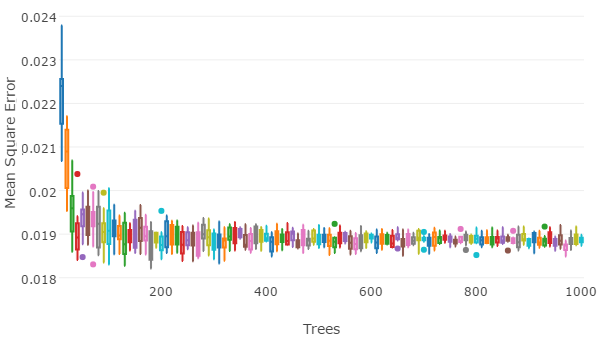
\includegraphics[width=\textwidth]{RF_analysis/mse_trees.png}
		\caption{Box plot : MSE with increasing number of trees}
		\label{} %  
	\end{subfigure}
	~~~~~~~~~~~~~~~
	\begin{subfigure}[t]{0.3\textwidth}
		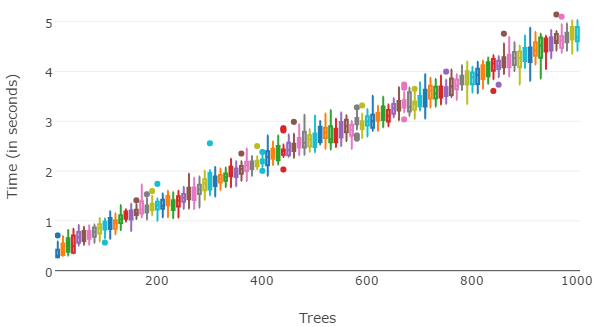
\includegraphics[width=\textwidth]{RF_analysis/timing_trees.png}
		\caption{Time with Trees increasing}
		\label{}
	\end{subfigure}
	\label{}
	\caption{Analysis of number trees in a Random Forest}
\end{figure}

A expected, the more trees, the smaller the MSE. Time is linear with number of trees, conformal to previous section analysis.


\subsection{Depth of the trees}

This parameter controls the data fit. Indeed, the deeper the tree, and the more over-fitted the model is. Inversely, the smaller the tree, the more under-fitted the model is. 
There is no theoretical value to take for the depth of a tree. Only analysis of the data can give an answer. Using a Cross Validation method can help figure out which value to take for this parameter. 

\begin{figure}[H]
		\label{figure:mse_leaves}
		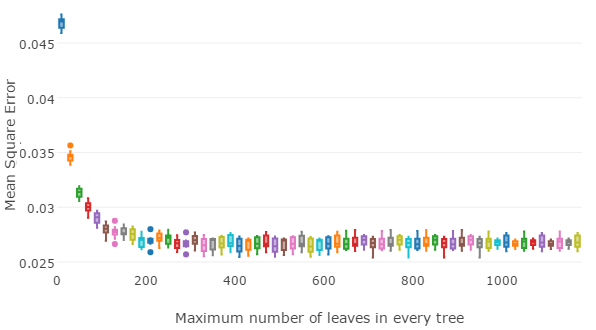
\includegraphics[scale=0.8]{RF_analysis/mse_leaves.png} 
		\caption{Box plot giving the mean square error given by Random forest with increasing number of leafs}
\end{figure}

For the Iowa data available with 1429 samples, taking more and more leafs and depth helps reducing the MSE. 

\subsection{Variable Importance and features selection} 


\subsubsection{Tuning the max\_features hyperparameter}

Without doubt the most efficient parameter for high dimensional computation is the number of features taken into account when generating a tree. 
Indeed, when growing multiple trees, one can limit to $K$ features, randomly chosen, and let the Random Forest process happens. Theory for this kind of feature selection in Random Forest is not abundant yet, but here is a quick analysis on our Iowa data of housing market.

\begin{figure}[H]
		\label{figure:mse_feature}
		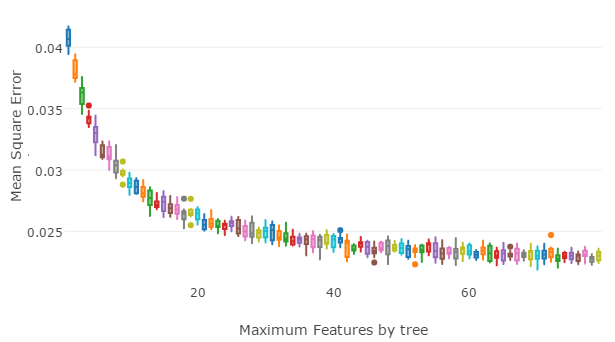
\includegraphics[scale=0.8]{RF_analysis/mse_features.png} 
		\caption{Box plot giving the mean square error of regression given by Random forest with increasing number of features}
\end{figure}


Of course, as expected, the bigger the number of features, the better the estimation. However, to get competitive time computation, one can prefer fewer precision, and limit to 40 features in this case, out of 79. 

Moreover, the previous graph provides a number of features chosen randomly between the 79 available. But, once can analyse the features first, and make a feature selection, explained in the following part.

\subsubsection{Selecting the best features : Variable Importance}

One can reduce the high dimensionality of a regression problem by selecting the 'best' features.

Measuring this so called \textit{Variable Importance} makes it possible to rank the features by their importance. The difficult part here is the way to measure a feature's impact on the regression model. 
Intuitively, the more an input $X_i$ is important, the worse the accuracy when removing it from the regression. 

Thus when training a tree, it can be computed how much each feature decreases the impurity in a tree, called impurity score and known as \textit{Gini impurity} for classification and variance for regression.

here method in \textit{Scikit-Learn} Random Forest Regressor class gives this information. 
Drawing in the previous example a variable importance histogram gives

\begin{figure}[H]
	\label{figure:vi}
	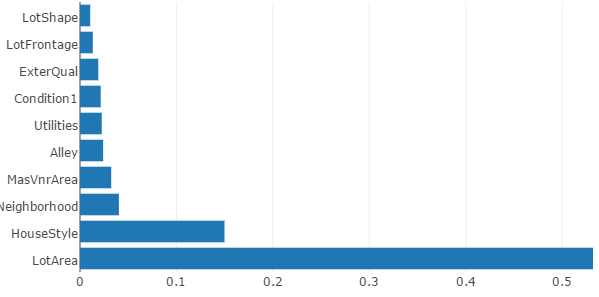
\includegraphics[scale=0.6]{RF_analysis/vi.png} 
	\caption{First ten most important variables given by Random Forest}
\end{figure}

Obviously the \textit{LotArea} represents the most important variable here.  



Had it been that easy, we would then select the best features and rerun a Random Forest. 
But, redundant information between features affects impurity measurements and thus its ranking. 
This is not an issue for prediction and avoiding over fitting, but can lead to misinterpretation about a label importance. 
\newline
For instance

\begin{Ex}
	let $X_0$, $X_1$, $X_2$,  $X_3$, $X_4$ and $X_5$ be six random variables having Gaussian distribution with mean 0 and variance 1.
	To add some correlation, we choose to add $X_0$ to every $X_i$,  $\forall i \in \{1,\cdots, 5\}$. 
	Let $Y$ be the sum of the correlated random variables $X_i$, $\forall i \in \{1,\cdots, 5\}$, i.e $Y = \sum_{i=1}^{5} X_i$. 
	It is clear here every input $X_i$ has the same impact on the output $Y$. 
	However, computing a Random Forest on $10.000$ samples of $(X, Y)$, $X$ being the concatenate of $X_i$, $i \in \{1,\cdots, 5\}$, gives the following Variable Importance bar plot
	\begin{figure}[H]
		\centering
		\label{figure:vi_ce}
		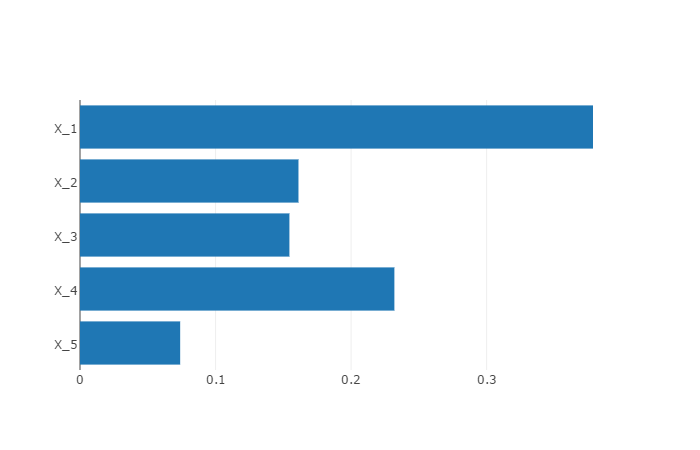
\includegraphics[scale=0.4]{RF_analysis/vi_contre_example.png} 
		\caption{Variable Importance with 5 correlated features $X_i$,$i \in \{1,\cdots, 5\}$ respectively taking importances 0.3785, 0.1612, 0.1545, 0.2319, 0.0739.}
	\end{figure}

	$X_1$ is five times 'more important' than $X_5$, which does not correspond to reality, as all inputs have the same impact on output $Y$. Random Forest seems to keep in 'mind' the information it gets, and if not needed, it does reduce its importance.  

\end{Ex}

Let's analyse this on the previous housing example :

First, let's draw the correlation matrix between the inputs (we draw only a part here for better visualization): 

\begin{figure}[H]
	\label{figure:correlation_matrix}
	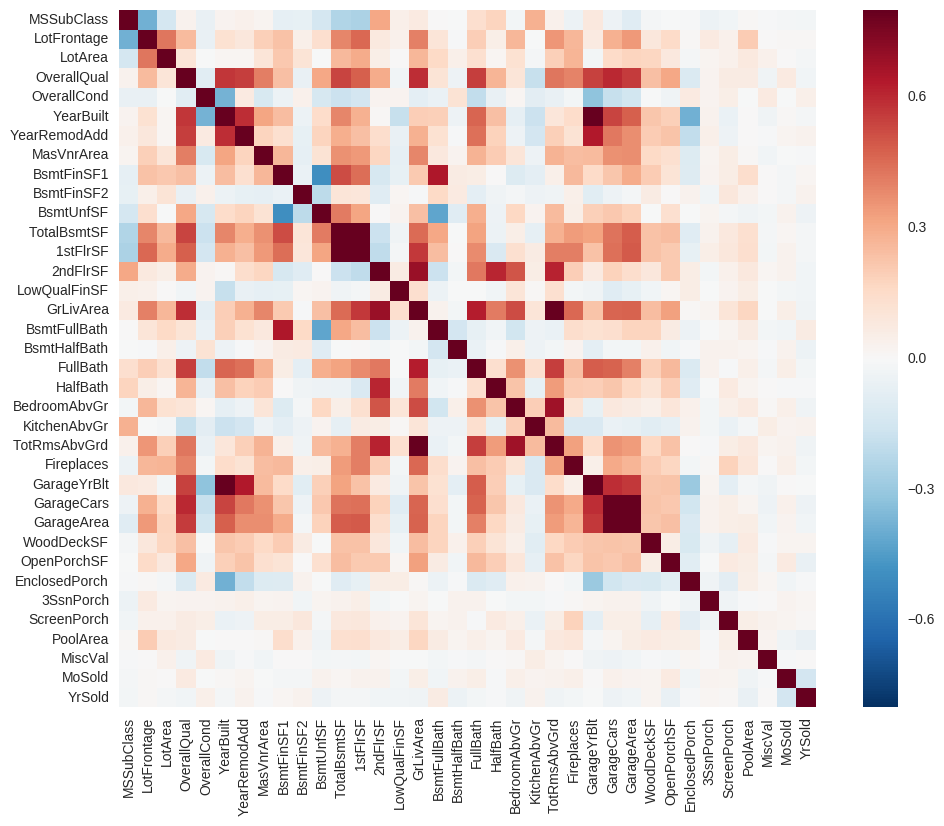
\includegraphics[scale=0.5]{RF_analysis/correlation_matrix.png} 
	\caption{Correlation matrix between the features of our housing market data}
\end{figure}

We can see \textit{LotFrontage}(Linear feet of street connected to property) and \textit{LotArea}("Lot size in square feet") are highly correlated (intuitively and by matrix correlation).
Growing a Random Forest gives the following Variable Importance ranking


\begin{figure}[H]
	\label{figure:vi}
	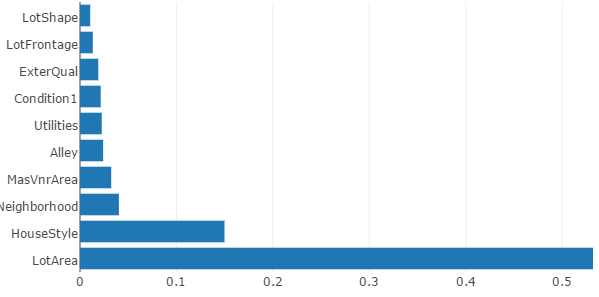
\includegraphics[scale=0.6]{RF_analysis/vi.png} 
	\caption{Correlation matrix between the features of our housing market data}
\end{figure}


The randomness of the algorithm managed here to make the best of both provided information in \textit{LotFrontage} and \textit{LotArea} and bucket it into the 'most important' one : \textit{LotArea}. 
Several analysis can be made on features to make the best selection, but this example illustrates how powerful Random Forest can be for regression problems...


\end{appendices}

\blankpage
\bibliographystyle{apa}
\bibliography{biblio}
% \bibliographystyle{plain}

\end{document}